\documentclass[conference]{IEEEtran}
\IEEEoverridecommandlockouts
%
\usepackage[table,xcdraw]{xcolor}
\usepackage[T1]{fontenc}
% T1 fonts will be used to generate the final print and online PDFs,
% so please use T1 fonts in your manuscript whenever possible.
% Other font encondings may result in incorrect characters.
%
\usepackage{graphicx}
\usepackage{esvect}
% Used for displaying a sample figure. If possible, figure files should
% be included in EPS format.
%
% If you use the hyperref package, please uncomment the following two lines
% to display URLs in blue roman font according to Springer's eBook style:
%\usepackage{color}
%\renewcommand\UrlFont{\color{blue}\rmfamily}
%\urlstyle{rm}
\usepackage{comment}
\usepackage{diagbox}
\usepackage{url}
%\usepackage{breakurl}
\usepackage[breaklinks]{hyperref}
\usepackage{graphicx}
\usepackage{bm}
\renewcommand{\vec}[1]{\bm{#1}}
\usepackage{subcaption}

\usepackage[utf8]{inputenc}
\usepackage[T1]{fontenc}
\usepackage{soul}
\usepackage{graphicx}
\usepackage{amsmath}
\usepackage{booktabs}
\usepackage{pifont}
\usepackage{enumitem}
\usepackage{tikz}
\usepackage{cite}
\usepackage{amsmath,amssymb,amsfonts}
\usepackage{algorithmic}
\usepackage{graphicx}
\usepackage{textcomp}
\usepackage{xcolor}
\usepackage{amsmath}
\def\BibTeX{{\rm B\kern-.05em{\sc i\kern-.025em b}\kern-.08em
    T\kern-.1667em\lower.7ex\hbox{E}\kern-.125emX}}
    
\def\checkmark{\tikz\fill[scale=0.4](0,.35) -- (.25,0) -- (1,.7) -- (.25,.15) -- cycle;} 
%shorten space between equation and text
\usetikzlibrary{trees,arrows}
\setlength{\abovedisplayskip}{4pt}
\setlength{\belowdisplayskip}{4pt}
\setlength{\abovedisplayshortskip}{4pt}
\setlength{\belowdisplayshortskip}{4pt}
%shorten space between figures and text
% Space between figure and text
\setlength{\textfloatsep}{6pt}
% Space between figure and caption
\setlength{\abovecaptionskip}{4pt}
\setlength{\belowcaptionskip}{4pt}
% Space between multiple floats
\setlength{\floatsep}{6pt}
% Space for in-text (here) figures
\setlength{\intextsep}{6pt}
% Space between table and surrounding text
\setlength{\textfloatsep}{6pt}
\setlength{\intextsep}{6pt}
\setlength{\floatsep}{6pt}
% Space between table and caption
\setlength{\abovecaptionskip}{4pt}
\setlength{\belowcaptionskip}{4pt}

\newlist{todolist}{itemize}{2}
\setlist[todolist]{label=$\square$}
\newcommand{\cmark}{\ding{51}}%
\newcommand{\xmark}{\ding{55}}%
\newcommand{\done}{\rlap{$\square$}{\raisebox{2pt}{\large\hspace{1pt}\cmark}}%
\hspace{-2.5pt}}
\newcommand{\wontfix}{\rlap{$\square$}{\large\hspace{1pt}\xmark}}

\def\UrlBreaks{\do\/\do-}

\renewcommand\thesection{\arabic{section}} % arabic numerals for the sections


% correct bad hyphenation here
\hyphenation{op-tical net-works semi-conduc-tor IEEEconf}

\begin{document}
%% Example cover page for a two-page IEEE conference document
%\onecloumn
% Cover page

\begin{center}
  \textbf{recovery testbed}
\end{center}

\begin{itemize}
  \item DEADLINE: Abstract April 11, Paper April 18, 2025
  \item Publication Venue: QEST+FORMATS 2025
  \item Url for Publication Venue: \url{https://www.qest-formats.org/}
  \item Submission Category or Track:
    \begin{itemize}
        \item Models and metrics for the correctness, performance, reliability, safety, and security of systems (stochastic, probabilistic, and non-deterministic models including Markov chains, automata, Petri nets, process algebra, max-plus algebra, and their variations);
    \end{itemize}
  \item Page limit:  16 pages; currently at 16
  \item Research Contribution: 
   The proposed model enables comparisons of alternative
repair schemes by considering the availability of repair crews,
predicting failure propagation, and estimating the level of
service capacity over time. The model can also guide staffing
decisions by identifying the minimum number of repair crews
required to maintain a particular service level.
\end{itemize}

\vspace{2ex}

%SSS- This helps us keep track of the number of drafts
\textbf{Version 1.1}
Last Updated: 4/1/2025 \\
\textbf{Major Changes Since Previous Draft}
\begin{itemize}
    \item Case study
    \item Conclusion
\end{itemize}

\vspace{2ex}

\textbf{Outline}
\begin{enumerate}
%SSS - Include the number of pages in your current draft in front of each section (not subsection) title. Also include the status (complete, pending, not written).
  %SSS - The following sections should be in every paper. 
  \item  Abstract
  \item Introduction 
  \begin{enumerate}
          \item Blackout in Kenya
          \item Motivation for this paper
          \item Intro to this model
        \end{enumerate}
  \item Related work
  \begin{enumerate}
          \item Modeling of cascading failure
          \item Modeling of the Recovery process
        \end{enumerate}
  \item Proposed recovery model
  \begin{enumerate}
          \item Modeling of Cascading failure
          \begin{enumerate}
              \item States
              \item Actions
              \item Rewards
              \item Transition probabilities
          \end{enumerate}
          \item Repair schemes
          \begin{enumerate}
              \item Randomized priorities
              \item pre-made repair priorities
              \item Look-ahead dynamic priorities
              \item cascading effect dynamic priorities
          \end{enumerate}
        \end{enumerate}
  \item case studies
  \begin{enumerate}
          \item IEEE-14
          \item Simulation Environment
          \item IEEE-14 Failure Cases
          \begin{enumerate}
            \item experiment 1
            \item experiment 2
            \item Experiment 3
            \end{enumerate}
        \item Discussion of results
        \end{enumerate}
  \item Conclusion and Future Work 
    \begin{enumerate}
          \item The contribution to the body of knowledge 
          \item social impact 
          \item future directions, enable advances in the repair scheme area
        \end{enumerate}
  \item Acknowledgements 
  %SSS - Include this text in your acknowledgments: The authors gratefully acknowledge funding from NSF DUE-1742523, DEd GAANN awards P200A180095 and P200A210121, and the Missouri S\&T Intelligent Systems Center.
  \item References
\end{enumerate}

\vspace{2ex}

\textbf{TO DO (Advisors):}
\begin{itemize}
    \item review the paper
\end{itemize}

\textbf{TO DO (Sanfan):}
\begin{itemize}
    \item review the paper entirely
    \item submit for publication 
\end{itemize}

\textbf{Author guidelines (submission requirements)}: \\ 
\url{https://www.qest-formats.org/cfp.html}\\
Regular papers must not exceed 16 pages, excluding references.
We are considering additional presentation-only submission types; details will be provided in the later CfPs.

All papers must be submitted in Springer’s LNCS format and will undergo a rigorous single-blind review process. All submitted papers must be unpublished and not be submitted for publication elsewhere. Papers should be submitted electronically using EasyChair at this link.

Springer encourages authors to include their ORCIDs in their papers. Authors should consult Springer’s authors’ guidelines and use Springer’s LaTeX templates for the preparation of their papers. Submitted papers not complying with the above guidelines may be rejected without undergoing review.
We are considering awards for best papers and best artifacts.

Publications\\
All accepted papers need to be presented and discussed at the conference by one of the authors. The QEST+FORMATS 2025 proceedings will be published in the Springer LNCS series indexed by ISI Web of Science, Scopus, ACM Digital Library, dblp, Google Scholar. All submitted papers will be evaluated by at least three reviewers on the basis of their originality, technical quality, scientific or practical contribution to the state of the art, methodology, clarity, and adequacy of references.

Special Issue\\
We are working on a special issue in a Q1 journal. A selection of the best papers will be invited to submit an extended version of their work to special issues in internationally recognized journals.

Artifact Evaluation\\
Reproducibility of experimental results is crucial to foster an atmosphere of trustworthy, open, and reusable research. To improve and reward reproducibility, QEST+FORMATS 2025 will include a dedicated Artifact Evaluation (AE). Submission of an artifact is mandatory for tool papers (both regular and short), and optional but encouraged for research and case study papers where it can support the results presented in the paper. More details can be found in the corresponding page
%End Cover Sheet



\title{RACE: Recovery Analysis for Cascading Events in Complex Networked Systems}



%SSS - add funding source for camera-ready
%\title{Personalizing Student Graduation Paths Using Expressed Student Interests
%{\footnotesize
%\thanks{Funding source redacted for double-blind review.}
%}}

%
%\titlerunning{Abbreviated paper title}
% If the paper title is too long for the running head, you can set
% an abbreviated paper title here


 %SSS - add in author info for camera-ready using COMPSAC template

\maketitle              % typeset the header of the contribution
%
\begin{abstract}
%SSS - add at least a bulleted outline  (SL: done)
This paper proposes a stochastic model that can guide recovery actions for tightly coupled systems where failure propagation may outpace recovery actions, leaving the system unable to provide even minimal service. 
To this end, we utilize a time-dependent Markov decision process (TD-MDP) to identify sequences of recovery actions that mitigate the effect of a detected failure on one or more aspects of system survivability. 
Efficacy of the proposed method is illustrated through case studies on smart grids based on the IEEE-14 and IEEE-30 test systems, where ...  A high-fidelity digital twin was implemented for each system  to accurately reflect component states and cascading dynamics. Simulation results indicate that the choice of recovery scheme can system survivability varies with initial failure conditions and resource availability, underscoring the importance of recovery scheme selection under different cascade scenarios. The results demonstrate that the TD-MDP framework supports  objective comparison of recovery strategies under consistent survivability criteria.
\end{abstract}

\begin{IEEEkeywords}
stochastic recovery model, Markov decision process, failure propagation, decision support, cascading failure, survivability
\end{IEEEkeywords}

%SSS - an attractive figure can hook in your reader and tell them that you know exactly what you are doing (SL: done)
\section{Introduction}
Cascading failures pose a significant hazard to the survivability of interconnected complex systems. The malfunction of a single component can trigger a chain of disruptions that propagate swiftly across interconnected subsystems. Such hazards can be found in many critical infrastructures, such as water distribution, urban transportation, and smart grids.

The consequences of cascading failures are severe, especially for infrastructures. They could delay restoration, increase economic penalties, and extend service interruptions. Predicting these consequences requires analytical frameworks that capture the dynamics of failure propagation and reflect the progression of repair. This paper seeks to elucidate the race between failure propagation and recovery actions intended to restore the system's functionality. We propose a mathematical model that helps identify the most prudent sequence of recovery actions given a specific objective such as maximizing the service capacity.

%SSS - Be consistent in using failure vs malfunction (SL: done)
An effective way to plan system recovery is to view it as a battle against the spread of failure. Functional interdependencies between components enable a failed component to bring down its ``neighbors''. Every additional failure, increases the likelihood of system collapse or catastrophic failure. However, all components are not equal. A ``critical'' component is one whose function or location in the system can make its failure especially consequential \cite{redacted}. Effective system recovery depends not only on rapid response, but also on identifying and prioritizing critical nodes. Poorly conceived recovery schemes, as illustrated by the 2023 Kenya blackout described below, have shown that the valuable time and effort spent on restoring non-critical components could lead to an otherwise preventable catastrophic failure. In contrast, the 2025 Spain blackout (also described below) demonstrates the value of a rapid and prudent recovery scheme.

The nationwide blackout in Kenya in 2023 underscores the severe consequences of ineffective recovery decisions. An error message at the Lake Turkana wind facility triggered the sudden loss of 270 MW of power, roughly 15\% of national demand. The recovery strategy was to stabilize the grid through importing power assumed to be available in Uganda, a neighboring country. Uganda's inability to deliver the required power made this an ineffective recovery scheme. More specifically, the decision to delay recovery of local systems allowed the outage to spread, eventually affecting close to 50 million people ~\cite{apkenya_aug23, apkenya_dec23, mwangi_kenya_2023}. 

In contrast, the 2025 Iberian Peninsula blackout highlights the value of a coordinated, knowledge-driven response. Operators activated cross-border interconnections with France and Morocco. An import of 2 GW of electricity from France (which in turn imported power from Germany) was sufficient to supply a few northern areas in Spain. Morocco transmitted 900 MW over Gibraltar to aid the southern region of Spain. These bilateral imports facilitated the reactivation of hydropower and gas turbine generators in Spain, enabling a progressive reestablishment of additional power generation units. Thereby limiting failure propagation and expediting recovery ~\cite{cetinkaya_technical_2025}. 

%SSS - The emphasis on interdependency should serve as a lead-in to explaining that your work is one of few studies that explicitly considers it (SL: as the foundation of our work)
Recent research has highlighted the role of interdependencies in the survivability of complex networked systems. Several studies have demonstrated that tight coupling between components can be a vulnerability. Measures such as redundancy, capacity enhancement, or load redistribution can improve survivability by slowing or halting cascades ~\cite{zhang_effects_2017}. However, these measures are often impractical given environmental limitations and the complex nature of actual systems; they may also fall short in averting widespread cascading failures, even in advanced smart grids. This underscores the significance of recovery schemes in mitigating the effects of such failures and maintaining uninterrupted service for users. Interdependencies should be considered in planning recovery actions, prioritizing critical components.

%main controbution
The broad goal of the research presented in this paper is to create mathematical models that enable better understanding of failure and recovery of a complex networked system. More specifically, our work aims to predict a) failure propagation among components, b) whether a given failure or sequence of failures will leave the system operational, and c) the impact of specific recovery actions, which allows the most prudent recovery plan to be identified. \emph{In short, we seek to elucidate the race between fault propagation and recovery actions and to identify the strategy that leads to the greatest resilience.}

Previous studies on recovery modeling fall short of enabling these goals. Unlike our proposed model, they assume that recovery is undertaken when the system is immune to additional failures, typically because it has been shut down for repair or isolation mechanisms are in place to prevent failure propagation. This is an unrealistic assumption for critical systems, as demonstrated by the blackouts in Kenya or Spain. Another shortcoming of these studies is imprecise or incorrect assumptions about recovery times \cite{sarkale_solving_2018, biswas_repair_2025}.
Our model reflects non-deterministic recovery times, with any probability distribution, broadening the applicability and increasing the accuracy of the model. 

More specifically, \textbf{the original research contribution of this paper is a mathematical model that reflects the operation of a complex networked system where recovery efforts are competing with failure propagation.} 

%SSS - give a quick explanation of MDPs and explain why they are a good choice here 
The basis is a Markov decision process (MDP) that reflects the state of both the system and the crews that can be dispatched to replace or repair failed components. The model can reflect a variety of recovery schemes and enable the identification of the ``best'' scheme, as evaluated by a quantitative measure of system-level functionality that changes as components fail or are recovered. Our work addresses a common shortcoming of related studies - the assumption that recovery times are fixed or exponentially distributed. Given that recovery is neither deterministic nor memoryless, our model better reflects reality by allowing any probability distribution to be used for recovery times. Time-dependent state transitions are key to this aspect of the model. 

To accurately reflect failure propagation, our model considers the interdependencies among the components of the networked system. Many studies have been identifying and quantifying these interdependencies and predicting failure propagation among interconnected components. Over time, failure propagation becomes less likely as failed components shut down or the system adapts to mitigate or isolate failure. In other words, the likelihood of failure propagation is highest when the triggering failure occurs and declines throughout the recovery process. Time-dependent state transitions allow our model to reflect this aspect of system failure and recovery. 

%What can others do with my research
Our work supports improved network design, efficient allocation of recovery resources, and the analysis, evaluation, and comparison of recovery schemes. 
For network designers, it assists in identifying improved topologies that enhance service delivery and expedite recovery from failure. Service providers can use our model to guide resource allocation, for example, to shorten recovery times for essential components. 
For researchers examining recovery schemes, this approach facilitates proactive planning by identifying robust recovery schemes ahead of disruptions, thus setting up efficient default procedures. It assists in prioritizing recovery tasks to make recovery more efficient and less costly. During an actual failure event, the model enables network operators to dynamically adjust recovery schemes and prevent catastrophic failure.

The insights gained from our model, like those from any other model, rely on the availability of reasonably accurate information about the system being modeled. As depicted in Figure \ref{fig:bigpic}, the model requires knowledge of the system's functional topology and component-level information about failure and recovery, respectively. Given this information, it can be used to evaluate and compare different recovery schemes. 

\begin{figure}
    \centering
    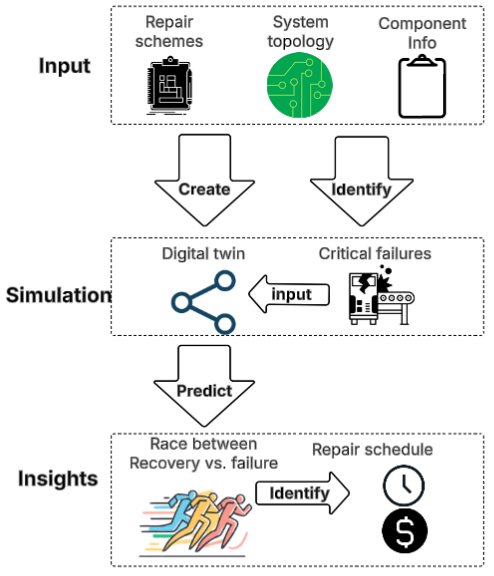
\includegraphics[width=0.5\linewidth]{images/BigPic.png}
    \caption{The data flow of our proposed model}
    \label{fig:bigpic}
\end{figure}

The remainder of this paper is organized as follows. Section 2 presents the related work in the field. Section 3 describes our methodology, the formulation of the model. Section 4 presents the case study conducted on standard IEEE bus systems. Section 5 concludes the paper. 
%Outline all sections here 

\section{Related work}
%To analyze the system during the cascading events, we must look at two particular topics. 
Given that the proposed model aims to capture the race between failure propagation and system recovery efforts, our literature review spans studies in the same two categories. The aim of the first category of related work focused on identifying dependencies is to understand and predict consequential failures that result from functional dependencies between components or subsystems. 
The second category of related work on recovery models for networked systems encompasses studies that share our goal of predicting the recovery process(from failure) for a given system and evaluating recovery schemes. 

Table \ref{tb:relatedModels} highlights the distinction of our work by comparing it to the studies discussed later in this section. 
\begin{table*}
\centering
\caption{Comparison of proposed approach to related work}
\label{tb:relatedModels}
\begin{tabular}{|l|l|l|l|l|l|}
\hline
\textbf{Study} &
  Failure prediction  method &
  Multi-layer system &
  Recovery model &
  Recovery time distribution &
  System performance metric(s) \\ \hline
\begin{tabular}[c]{@{}l@{}}This \\ research\end{tabular} &
  \begin{tabular}[c]{@{}l@{}}Dependency based\\ probability\end{tabular} &
  \checkmark &
  \checkmark &
  \textbf{Any} &
  \begin{tabular}[c]{@{}l@{}}Restoration time, additional \\ failure, survivability\end{tabular} \\ \hline
Ref \cite{zhang_cascading_2021} &
  \begin{tabular}[c]{@{}l@{}}Coupling \\ relationship\end{tabular} &
  \checkmark &
   &
   &
  Power load loss rate \\ \hline
Ref\cite{xu_cascading_2024} &
  Capacity overload &
  \checkmark &
   &
   &
  \% of nodes lost \\ \hline
Ref\cite{sarkale_solving_2018} &
  None &
   &
  \checkmark &
  Exponential distributions &
  Number of users receiving service \\ \hline
Ref\cite{yan_dynamic_2021} &
  None &
   &
  \checkmark &
  Weibull distribution &
  System functionality lost \\ \hline
Ref\cite{biswas_repair_2025} &
  None &
   &
  \checkmark &
  Fixed &
  Total service disruption time \\ \hline
Ref\cite{wang_q-learning-based_2025} &
  Dispersion probability &
  \checkmark &
  \checkmark &
  1-time step &
  Power supply \\ \hline
\end{tabular}
\end{table*}
\subsection{Related work in cascading failure}
The research reviewed in the first category aims to identify and quantify the vulnerabilities and dependencies within complex networked systems. 
%measuring dependency in general system (from occurance of consequencial component failures)
%The common objective of these researches is to comprehend the dynamic effects of failure propagation, e.g., predict the consequences of a given initial failure. 
From observing the system behavior in past failure events, the interdependencies between component A and component B can be measured with mathematical metrics or models.
For instance, Pearson correlation ~\cite{modarres_measures_2011} is a measure of the mutual dependence between two variables; it captures the linear association between the occurrence of two events. Which can be used to measure the probability that the failure event of one component can lead to the failure of the other from past failure events without limitation of the type of system. Similarly, Spearman's rank correlation ~\cite{modarres_measures_2011} measures the monotonic relationship by using rank values between two variables and is often compared with Pearson correlation, as it captures nonlinear relationships that Pearson correlation was unable to. Randomized Dependence Coefficient ~\cite{lopez-paz_randomized_2013} is another measure of nonlinear dependence between random variables that can apply to arbitrary dimension, with a low computational cost for large systems with many components. 
%measure in specific system
Specialized research has been conducted to quantify dependencies in various types of systems. For instance, hydraulic criticality measures~\cite{marlim_hydraulic_2024, jeong_comparative_2020} quantitatively assess failure propagation within water distribution networks using pipeline water pressure measurements, which can help detect uneven pressure distribution and potential pipe bursts.

In traffic systems, spatial-temporal correlation~\cite{du_novel_2021} and Granger causality~\cite{hasan_analysing_2016} are employed to evaluate traffic conditions, considering meteorological factors, vehicular speed, traffic flow, and vehicle density. These factors affect the likelihood of traffic congestion and vehicular accidents.


Cascading failures in electrical power systems, particularly those caused by capacity overload, have been analyzed using graph theory and heuristic models~\cite{xu_cascading_2024, yan_dynamic_2021, zhang_effects_2017, zhang_cascading_2021, nyberg_failure_2015, redacted}. These failures occur when redistributed subsystem loads exceed component capacities, triggering automatic shutdowns or even transformer fires. Similar approaches have been applied to port logistics systems, where demand exceeding capacity can result in significant operational disruptions~\cite{wang_resilience_2026}.

%conclusion and why is our work useful (I got it from QEST paper)
These studies, among others, show that the dependencies between components are measurable, which gives us a chance to predict and prevent the cascading failure from happening. However, due to the complexity of the system, cascading failure will still happen to the system. Therefore, our proposed model goes further by reflecting on and enabling analysis of the effects of recovery efforts undertaken concurrently with a cascading failure. This work builds on the method proposed in \cite{redacted} that created a dependency index to represent the conditional probability of failure propagation between components of a cyber-physical system. 

\subsection{Related work in recovery models}

The second category, studies related to the recovery model, typically focuses on comparing recovery schemes or introducing a new scheme. The standards used often involve a comparison of system performance and functionality during the recovery process. The goal is to identify a scheme that enables the quickest recovery of system performance or reduces the cost for recovery or loss of service (penalties).Notable work in this category includes studies by Sarkale et al. ~\cite{sarkale_solving_2018}, Yan et al. ~\cite{yan_dynamic_2021}, Biswas et al. ~\cite{biswas_repair_2025}, and Wang et al. ~\cite{wang_q-learning-based_2025}, where a mathematical model has been applied to power and water systems. 

The goal is to identify the dynamic repair scheduling algorithm with the highest recovery rate. The model proposed in Sarkale ~\cite{sarkale_solving_2018} and Yan ~\cite{yan_dynamic_2021}'s work aimed to identify the recovery scheme that could recover the system functionality the quickest in a post-hazard scenario. 
%detail explaination
In Yan's method, the extent of lost functionality is the basis for estimating performance, and the scheme chosen is the one that recovers the most functionality. In contrast, the number of users who continue to receive service is the basis for comparison in Sarkale's method. 
Lin et al. \cite{lin_condition-based_2022} proposes an  Markov decision process(MDP) model for the maintenance of power supply equipment, where the goal is to minimize the sum of penalties and repair costs and reduce the cost of upkeep in the long run. 

Similar to Yan and Sarkale's approach, Biswas's~\cite{biswas_repair_2025} model also assumed a post-hazard scenario; however, it assumed that the exact location of the failure is unknown and requires the crews to search approximated failure areas before they can begin repairs. This adds a path-finding problem on top of the recovery scheme. 

%Wang's model~\cite{wang_q-learning-based_2025} is much closer to our work, as it predicts the failure propagation of the network from the initial failure and then begins the recovery task scheduling for the crews. Compared to the three others, Wang's model was able to produce a recovery estimation considering cascading failures, but didn't show any ability to schedule the recovery schemes to mitigate the cascade, as the repair only begins after the failure is done propagating. Also unrealistic that recovery usually begins whenever disruption is detected, not when it's done propagating. 

The closest work to ours is Wang et al. proposed a cyber-physical power system model to test their Q-learning-based recovery method in \cite{wang_q-learning-based_2025}. The proposed model was developed to analyze the coupling between components within a Cyber-Physical Production System (CPPS) and to forecast potential failures before the initiation of recovery protocols. The findings indicated that their approach offers a more accurate representation in identifying potential cascading failures. Nonetheless, recovery processes are typically initiated following the first detection of disruption. These processes generally commence before the failure has fully propagated, thereby allowing a temporal advantage to mitigate its impact.

On the other hand, Wang's model\cite{wang_q-learning-based_2025} assumes that all recovery tasks require an identical duration, which constitutes a highly problematic assumption. While Biswas's \cite{biswas_repair_2025} model have assumed fixed, known recovery times. They may be adequate for crude timescales (measured in days). The urgency of preventing failure propagation necessitates a finer timescale (minutes or hours) for recovery actions. Deterministic recovery time is an unrealistic assumption on these finer time scales. Sarkale's model ~\cite{yan_dynamic_2021} assumes an exponential recovery time, which is somewhat more suitable for the timescales; however, having an exponential distribution alone is insufficient. a complex system consists of various types of components across multiple layers could have different recovery time distributions. For example, a smart grid usually contains electrical parts that deliver power to the physical layer, the recovery time distribution for physical parts is usually Lognormal ~\cite{l_c_cadwallader_review_2012} distributions, depending on component complexity and safety protocols for crews.  There is also cyber layer in the smart grid that contains smart meters and controlling devices to stabilize the power flow.The recovery time distribution for cyber is usually an exponential distribution that can be mostly done by rebooting in a short time (<5 mins), or requires a replacement like a physical component.

%Add a final wrap up of this section
Ultimately, this modeling framework aims to establish a mathematical foundation for decision support in recovery operations, facilitating the identification of optimal recovery strategies under varying failure scenarios and resource constraints.

The model accommodates inhomogeneous recovery‑time distributions, affording the flexibility necessary to represent structurally and functionally complex networked systems across diverse domains rather than being constrained to a single network type or network layer. Moreover, it is readily transferable to additional infrastructure systems—such as water, gas, and data networks—and enables systematic examination of recovery across multiple interdependent layers, including both physical and cyber domains.


\section{Methodology}

%SSS - all of your reasons for choosing a Markov model, MDP, TI, specific prob distr need to be crystal clear. Basically address the QEST comments with surgical precision. 
This section introduces our proposed model, the formulation of a Markov Decision Process (MDP) model with time‑dependent transitions to capture both interdependencies and recovery efforts. The goal is to characterize failure and recovery efforts in complex networked systems by predicting component and crew states, tracking failure propagation and recovery, assessing impacts on system survivability, and evaluating recovery schemes to inform optimal restoration strategies. To provide context, we present the model’s conceptual scope along with the underlying assumptions below:
\subsection{Assumptions}
\begin{enumerate}
    
    \item \textbf{Failure Dynamics:}Within each simulation time step, multiple components may fail or recover as failures occur, propagate through network interdependencies, and are resolved through restoration efforts. Failure propagation is represented as a stochastic process determined by component-specific failure rates and interdependencies among system elements,  enabling a realistic depiction of cascading failures at the system level. \label{assumption failure}

    \item \textbf{Failure Scope:}At the current stage, the model focuses exclusively on cascading failure dynamics triggered by specified initial failure scenarios. Random, self‑spontaneous, or independent failures are outside the scope of the present study and may be incorporated in future work to extend the framework toward more general reliability analysis.\label{assumption scope}
    
    \item \textbf{Observability of components :}All system components are assumed to be observable to the decision maker either directly or through sensor outputs transmitted to the control center. This ensures continuous awareness of system state even in cases where direct monitoring is not feasible, providing timely and accurate information for operational decision‑making. Several recent studies demonstrated the utility of wireless communication, sensors, and monitoring systems in detecting component-level failures in a smart system \cite{aust_performance_2012, verma_wireless_2014, tashtarian_distributed_2018}. \label{assumption:obser}

    \item \textbf{Flexibility of recovery time :}Recovery duration is modeled using empirical distributions derived from historical maintenance records, incident reports, and operational logs with time-dependent transitions to extend beyond fixed or exponential assumptions. The model captures variability arising from severity of failure, resource allocation efficiency, and environmental conditions and defines recovery time to include logistics, repair work, boot‑up, verification, and testing since all steps require the continued presence of crews at the component site.
     \label{assumption:repairt}
    
    \item \textbf{Success of recovery :}Every failed component is assumed to be recoverable, with restoration always succeeding through either repair or replacement. This simplifying assumption enables clear interpretation of results and can be relaxed in future works.

    \item  \textbf{Recovery resources :}Restoration activities rely on a fixed number of repair crews available throughout the entire recovery process. Each crew is capable of executing any required repair or replacement task but is limited to one assignment at a time, establishing a realistic yet tractable representation of resource constraints.

\end{enumerate}

Collectively, these assumptions establish a modeling standard that enables a more realistic simulation of a complex networked system and preserves the essential dynamics of failure propagation and restoration. They allow the model to focus on comparing the recovery schemes in a practical setting. At the same time, these assumptions highlight opportunities for future model extensions, %including partial observability, probabilistic repair success, and heterogeneous recovery crews,%
allowing gradual relaxation of assumptions as data and computational resources permit.

\subsection{Model formulation}
A Markov decision process (MDP) is a state-based model for sequential decision-making when actions can have uncertain outcomes. An MDP has four elements:
%SSS - reconcile with 6440 notes 
\begin{itemize}
    \item A set of states, $S$
    \item A set of transitions $P$
    \item A set of actions, $A$
    \item A set of rewards, $R$
\end{itemize}

\subsubsection{System state \texorpdfstring{$S$}{S}}
The state occupied by the MDP at a given decision epoch is determined by the respective states of the components and the crews.

The \emph{components} are defined at a granularity that allows the state of each component—either \emph{operational} or \emph{failed} - to be directly observable, consistent with Assumption \ref{assumption:obser} (Observability of Components). If a component is failed, the failure time will be recorded in the state of the component for calculating time-dependent transitions. The state of the component, $x_i$, is determined as in equation \ref{eq:xs}, where all components are assumed to be functional at startup, i.e., $t_{fi}>0$ for all $i$.
\begin{equation} x_i (t)= \begin{cases}
    0 & \text{if component \textit{i} is operational}  \\
    t_{fi} & \text{if component \textit{i} has failed at time $t_{fi}$}
    \label{eq:xs}
\end{cases}\end{equation}

For a complex networked system with a total of $N$ components, the system-level state is represented by the vector $\mathbf{x}$, as in equation \ref{eq:X}.
%a.r. where xi is the state of component i
\begin{equation}
\mathbf{x} (t) = \{ x_1, x_2, \ldots , x_N \}
\label{eq:X}
\end{equation}

Crews are the second aspect involved in identifying the state of the recovery process at a given decision epoch. Each crew, $k$, can be either ``idle'' or busy recovering a particular component. The corresponding state, $y_k$, can be determined as shown in Equation \ref{eq:ys}, where $i$ represents the failed component that is assigned to crew $k$ for recovery. 
\begin{equation} y_k (t)= \begin{cases}
    0 & \text{idle, no recovery task assigned} \\
    i & \text{taking recovery actions on component $i$}
    \label{eq:ys}
\end{cases}\end{equation}

Assuming a total of $M$ crews available for dispatch, the state of the crews is collectively represented by the vector $\mathbf{y}$, as in equation \ref{eq:Y}. 

\begin{equation}
\mathbf{y}(t) = \{ y_1, y_2, \ldots , y_M \}
\label{eq:Y}
\end{equation}

Other than tracking the failed components that each crew is recovering, the time remaining to complete the recovery task is also tracked in an array with a length of $M$. Each $z_k$ should contain an integer that represents the remaining recovery time for the corresponding crew $k$ in crew state $\mathbf{y}$:
$$z_k (t)= \text{remaining recovery time of crew } k$$
\begin{equation}
    \mathbf{z}(t) = \{z_1, z_2, z_3 .., z_M\}
    \label{eq:z}
\end{equation}


Combining the component states in equation \ref{eq:X} and the crew states in equations \ref{eq:Y} and \ref{eq:z}, we obtain the system state, as illustrated in equation \ref{eq:S}
\begin{equation}
    \mathbf{S}(t) = \{\mathbf{x}(t),\mathbf{y}(t), \mathbf{z}(t) \}
    \label{eq:S}
\end{equation}
%To extinguish the system state at different time steps over the horizon, variable $t$ is assigned to identify system state at different time steps, as in the equation \ref{eq:St}
%\begin{equation}
%    S(t) = \{\mathbf{x}(t),\mathbf{y}(t)\}
%    \label{eq:St}
%\end{equation}

\subsubsection{Time-dependent transitions \texorpdfstring{$P$}{P} }
In a Markov decision process model, transitions $P$ determine the probability of the system entering the next state $S(t+1)$ as time increases. In our model, the transitions are dominated by two different processes: cascading failures and recovery efforts. The former transition is passively determined by the dependencies between components. And the later transition is controlled by actions $A$ that are motivated by rewards $R$. They will be explained, in order, in the following section. 

\paragraph{Cascading failure} 
A component can transition from ``operational''  to  ``failed'' due to independent failure or dependency on a failed component. The probability of the latter is quantified by the dependency index articulated in \cite{redacted}. For a system with $N$ components, the dependency indices can be represented by a matrix $D$:
\begin{equation}
D=[d_{ij} ] \in [0,1]^{N \times N},  
\end{equation}
$$i \in [1, N], j \in [1, N]$$
$d_{ij}$ represents the conditional probability of component $j$ failing one time step after component $i$ has failed. The heuristic causation analysis we used to compute the value of each element in $D$ is described in detail in  \cite{redacted}. Other ways to measure dependencies are mentioned in the related work section.% e.g., methods proposed by Qi et al. \cite{qi_interaction_2015} can also be used to populate $D$.

Then, we normalize $\mathbf{D}$ by dividing it by $N$ to ensure that $\sum^{n}_{j=1}d_{ij} \leq 1$. The matrix $\left( \frac{1}{N} \mathbf{D} \right)^l$ is then used to predict the probability of failure propagation from each component to every other component after $l$ time steps. Given the state of component $i$, the probability that component $j$ will fail in the next time step in a cascade from $i$ is a conditional probability shown in equation \ref{eq:pij}
\begin{equation}
p_{ij}(t) = \begin{cases}
    0 & x_i = 0 \\
    d_{ij} \in \left( \frac{1}{n} \mathbf{D} \right)^{(t-x_i)}    &x_i \neq 0
\end{cases}
\label{eq:pij}
\end{equation}
Note that $t$ represents the current time, and $x_i$ is the failed time of the component $i$, as described in equation \ref{eq:xs}. 
To find the total cascading effects on component $j$, a summation from every component in the system must be calculated, as shown in equation \ref{eq:c}, which represents the time-dependent transition for component $j$ from operational $(x_i(t) = 0)$ to failure $(x_i(t+1) = t+1)$ as a result of the cascade.

\begin{equation}
P_j(t)= \sum_{i=1}^{N} p_{ij}(t)
    \label{eq:c}
\end{equation}

\paragraph{Component recovery}
is the opposite of failure; that transition involves a component moving from failed $(x_i(t) =t_{fi})$ to operational $(x_i(t+z_k) = 0)$ via recovery efforts by crew $k$. As stated in assumption \ref{assumption:repairt}, the recovery is always successful; however, the time required for recovery is uncertain and is presented as a distribution function $f_i(t)$ for the component $i$. We must find the cumulative distribution function (CDF) of the recovery time $F_i(t)$. Then, a random variant is drawn between 0 and 1, 
and the determined recovery time $(t_{ri})$ of the failed component $i$ will be calculated based on the inverse function of the random variable:
\begin{equation}
    \text{Recovery time of }i :t_{ri} = \lceil F_i^{-1}(\text{Uniform}(0,1)) \rceil
    \label{eq:tri}
\end{equation}
It will be rounded up to the nearest integer for a discrete-time model and stored for the remaining task time for crew $k$. $\mathbf{z}$ will decrement as the time step moves forward $\mathbf{z}(t+1) = \mathbf{z}(t) - 1$. When an element $z_k$ reaches 0, the component is recovered $x_{y_k} = 0$, and then the crew $k$ will enter the idle state $y_k = 0$ in the next time step, ready for a new recovery task.

\subsubsection{Actions \texorpdfstring{$A$}{A} }
%How to address general repair distribution with TI
Action space $\mathbf{A}$ is the set of actions available to the system at a given decision epoch. Each action allows the agent to alter the transition or bring the system to a new state. 

In our model, the agent represents the decision support of the recovery process, mimicking the decision-making process of the network operators. the action space is finite and countable; each action represents assigning a failed component  $i | (x_i \neq 0)$  to an idling crew $k | (y_k = 0)$ for recovery. This condition can be expressed as shown in Equation \ref{eq:feasible}. 
\begin{equation}
(\exists i \in [1,N] | x_i \neq 0) \land (\exists k \in [1,M] | y_k = 0)
\label{eq:feasible}
\end{equation}

At each epoch, the agent will assign all the failed components to idle crews, based on the given recovery scheme, and continue until one of them (idle crews or failed components) is depleted. Two crews cannot simultaneously recover the same component, i.e., for every $x_i \in \mathbf{x}$ where $x_i \neq 0$, there is at most one $y_k \in \mathbf{y}$ where $y_k = i$. The assignment of an action to a crew will cause a transition in the next time step from ``idle'' to $i$, reflecting the component being recovered by the crew. Its corresponding recovery time tracker $z_k$ will be assigned a new value found using equation \ref{eq:tri}, given $i$'s historical recovery time. Scheduling of recovery actions is non-preemptive; i.e., a crew will remain on a given task until its completion. 

%SL: Major change to reawrds as well (compare to QEST) 
\subsubsection{Rewards \texorpdfstring{$R$}{R}}
\label{sec:rewards}
In traditional MDP, reward is a value generated for each action to compare its effectiveness, usually with a positive impact on the system, or to reduce the penalties to the system. 

In our model, the rewards will be used to evaluate the recovery schemes instead, so they can be compared. The common ways to compare the recovery scheme are usually their ability to minimize recovery time \cite{biswas_repair_2025}, minimize failures \cite{wang_q-learning-based_2025}, maintain the service capacity \cite{redacted3,yan_dynamic_2021,sarkale_solving_2018}, and meet a specific recovery deadline.  The rewards for each scheme will be averaged across multiple simulation trials to facilitate an average comparative analysis.

Success in \emph{minimizing recovery time} can be assessed by the earliest time that the system reaches the state where every component is operational, as shown in equation \ref{eq:ERT}.
\begin{equation}
    \text{earliest restoration time, } t, \text{ when }
    \mathbf{x}(t) = \{0,0, ... , 0\}
    \label{eq:ERT}
\end{equation}

The success in \emph{minimizing failure propagation} can be assessed by calculating the total number of additional failures triggered by the initial failure, i.e., the total number of transitions out of the $x_i(t) = 0$ state, for all $i$. Beginning the count $t=2$ excludes the triggering (initial) failure from the sum.
\begin{equation}
    \text{additional failures} = \sum_{i=1}^{N}\sum_{t=2}^{t=\infty} \mathbf{S}\{\mathbf{x}_i(t-1) = 0, \mathbf{x}_i(t) \neq 0\} 
\end{equation}

Success in \emph{Maintaining service capacity} can be measured by evaluating survivability of the system by determining the fraction of full service capacity delivered in a given state. This is shown in Equation \ref{eq:SC}
\begin{equation}
    \text{survivability(t)} = \frac{\text{ service capacity at }\mathbf{x}(t)}{\text{service capacity of } \mathbf{x} = \{0,0 ...0\}}
    \label{eq:SC}
\end{equation}

The success in \emph{meeting the recovery deadline} can be measured by evaluating the System survivability after a certain time step. Because many electric utilities operate under strict reliability and restoration deadlines, prolonged power outages can have severe consequences. Perishable food items in supermarkets may begin to spoil within a few hours, and residential buildings can lose their internal thermal stability within approximately 8–12 hours in cold climates\cite{noauthor_how_nodate}`. Under extreme conditions, such loss of heating can be life-threatening, as evidenced by the fatalities reported during the 2021 Texas power crisis~\cite{svitek_texas_2022}.

\section{Case study}
%add intro here
To demonstrate that our recovery model effectively captures the dynamics of a complex networked system, particularly the competition between failure propagation and recovery efforts, we adopt a smart grid as the case study for its relevance, clarity, and scalability. Specifically, respective smart grids are created from the IEEE-14 and IEEE-30 test systems, which include physical components such as power generators, buses, and transmission lines; by supplementing them with a cyber layer that incorporates phasor measurement units (PMUs) that are high-speed sensors that carry out time-synchronized monitoring of voltages and currents \cite{asprou_optimal_2011}, flexible AC transmission systems (FACTS) for control power flow and increase stability \cite{sosnina_assessment_2022, garrido_location_2019}, and  decision support (DS) that determine optimal settings for the FACTS device based on data from the PMUs. 

Four recovery schemes are evaluated against representative failure scenarios commonly observed in these test systems. Detailed information regarding the software implementation and validation of the proposed model is presented in this section.

The failure scope of the case study is focusing on the transmission lines, as they have higher failure rates as compared to other components and are often the cause of power outages \cite{song_survey_2013}. Along with the failures of cyber components, i.e., PMUs, FACTS devices, and the decision support system, is also considered, as their malfunction can lead to cascading failure in an otherwise stable grid \cite{redacted2}. 

\subsection{recovery scheme tested}
We demonstrate the recovery model by applying it to the four recovery  schemes described below, which differ in how they prioritize components for recovery. 

\begin{enumerate}
\item \textbf{Randomized} scheme randomly selects a failed component at each decision epoch and assigns it to an available crew for recovery. 

\item \textbf{Pre-computed} scheme selects a failed component at each decision epoch following a static list that is computed beforehand, with priorities determining the order of repair when multiple components have failed. The priorities can be ranked based on various metrics—such as the number of connections, service capacity, etc. In our case study, we constructed the priority list according to the total influence a component can bring to others when it fails. It was calculated by summing the row of the component in the dependency matrix $\mathbf{D}$, shown in equation \ref{eq:precomputed}
$$
\text{importance of component } i = \mathbf{D}_i = \sum_{j=1}^{N} d_{ij}
\label{eq:precomputed}
$$

\item \textbf{Max-capacity} scheme is a dynamic prioritization algorithm that selects a failed component at each epoch. The algorithm observes the component level state $\mathbf{x}(t)$ and develops a priority list of the failed components, assigning them to idle crews until one of them is exhausted.

This scheme was adapted from Yan at el. \cite{yan_dynamic_2021} that aims to increase service resilience by prioritizing the repair of components that achieve the greatest recovery rate for service capacity. Using the survivability equation \ref{eq:SC}, find the highest system survivability after each failed component has been repaired. 
For example, if components $i$ and $j$ have failed in the current state $\mathbf{x}(t)$, we need to compare survivability achieved by respective prioritization of the recovery of $i$ and $j$.The one with higher survivability bounce-back will be assigned to the idle crew. In situations where more than two components have failed, the algorithm will generate a list and  assign the task from the highest survivability bounce-back on the list to lower values. 

\item \textbf{Min-cascade} scheme also creates a dynamic list and assigns the tasks to idle crews. The only thing different here is the metric used to create the list. This scheme aims to lower the overall dependencies in the system by repairing the components that have a lower repair time and a higher probability of causing others to fail. As shown in equation \ref{eq:min_cascade}, a value for each component is calculated by dividing the sum of out-degree dependency of the failed component $i$ by its expected repair time. Then, a list can from sorting the 
\begin{equation}
\label{eq:min_cascade}
\text{cascading index of } i 
= \frac{\sum_{j=1}^{N} P_{ij} (t)}{E[t_{ri}]}
\end{equation}

\end{enumerate}

\begin{table}
\centering
\caption{Summary of recovery schemes}
\label{table:recovery}
\begin{tabular}{|l|l|l|}
\hline
\textbf{Schemes} & \textbf{Order of recovery tasks} & \textbf{Expected outcome} \\ \hline
\textbf{Rand}omized       & Random                           & Random outcome            \\ \hline
\textbf{Pre-com}puted &
  \begin{tabular}[c]{@{}l@{}}Computed beforehand to \\ minimize failure\end{tabular} &
  \begin{tabular}[c]{@{}l@{}}Lowest additional \\ failures\end{tabular} \\ \hline
\textbf{Max-cap}acity &
  \begin{tabular}[c]{@{}l@{}}Dynamically maximize \\ recovered capacity\end{tabular} &
  \begin{tabular}[c]{@{}l@{}}Highest survivability \\ in early stage\end{tabular} \\ \hline
\textbf{Min-cas}cade &
  \begin{tabular}[c]{@{}l@{}}Dynamically minimize \\ failure propagation\end{tabular} &
  \begin{tabular}[c]{@{}l@{}}High recovery \& \\ low additional failure\end{tabular} \\ \hline
\end{tabular}
\end{table}
\subsection{ Simulation software setup }
%SSS - mention that data sets, code, etc. are publicly available for reuse
Our experiments were carried out using fault injection on PSAT ~\cite{psat_2005}, an open-source MATLAB-based toolbox for power system analysis, which we have modified to allow simulation of interactions between components such as PMUs and the decision support algorithm that identifies the settings for the FACTS devices. Paper \cite{redacted4, redacted}  describes the simulation environment and explains how cyber-physical interdependencies are quantified. 
Simulation software was implemented in Python 3 on Google Colab \cite{colab}, with three inputs: i) the dependency matrix, ii) recovery time, and iii) an algorithm or a search table to assess the survival of the system.

\paragraph{i) The dependency matrix} $(\mathbf{D})$ governs the transition probabilities and reflects cascading failure. As described in the related work section, this value can be calculated using various methods for different types of complex systems. For our experiment, the dependency matrix for IEEE-14 and 30 smart systems was calculated using the method proposed in \cite{redacted}. %For better observe of the failure propagation in the system, we amplify the matrix calculated by $\mathbf{D} = \mathbf{D}^\frac{1}{2.5}$, so the value will exceed 1.

\paragraph{ii) Recovery time}
The recovery time for transmission lines was assumed to range from 3 to 7 hours in a lognormal distribution after recent studies on the repair time of physical components \cite{zapata_repair_2008, arif_optimizing_2018}. For smart devices, the total recovery duration is assumed to be 1 to 3 hours in exponential distribution, since the Department of Energy claims that they can reboot from a distance in < 5 min, or if someone needed to replace the device, we still need to round it up to the nearest integer, and the replacement time would have to include overhead time in preparation, travel, and installation \cite{noauthor_recovery_nodate, arif_optimizing_2018}.

\paragraph{iii)  An algorithm or a search table for assessing system survivability} A fundamental function required of a smart grid is the reliable delivery of uninterrupted electrical power to end users. In our case, the survivability assessment scale for the smart grid is judged by the number of power loads in the system that has been provided with adequate power. Consistent with standards such as EN-50160, we assess whether a load is considered supplied by verifying that the voltage of the BUS to which the load is connected is within a specified admissible interval. As an illustration, EN-50160 defines this interval as 0.9 to 1.1 per unit, where the per-unit quantity corresponds to normalization regarding a reference value, in this context a nominal voltage.


\textbf{Recovery simulations terminate} upon full system restoration or upon reaching a predefined simulation horizon. The finite horizon reflects practical recovery windows and avoids unrealistically long recovery realizations. The percentage of runs that complete recovery within the horizon is recorded as an additional recovery performance metric, while incomplete runs are treated as the earliest restoration time = the last time step on the horizon. Another reward,\emph{coverage} is added to the result collection that represents the \% of simulation completed within the time horizon. 

\subsection{Results: IEEE-14 \& 30}
The IEEE‑14 system is used for a detailed examination of the recovery process and comparison between multiple scenarios in multiple simulations. The IEEE‑30 system is used to demonstrate scalability, validating that the proposed testbed and modeling assumptions can be extended to larger and more complex network topologies. A search table is used to speed up the system by assessing the system survivalbility for when the system has $\leq 3$ failed lines. And the survivability will be 0 when there are more than 3 failures, because 3+ line outages can certainly collapse the system, and the power flow may not be solvable. The recovery recovery are chosen to have recovered at least 90\% of the system survivualbility by the 11th time steps (chosen from the range provided by House thermal stability \cite{noauthor_how_nodate}).

The original IEEE-14 includes 5 generators, 20 transmission lines, 14 BUS, and 11 loads. We have created an IEEE-14 smart grid from the original physical system by adding 3 PMUs,  3 FACTS devices, and a decision support system. The PMUs were placed on BUS 2, 6, and 9, respectively. These are the locations identified in a study by Asprou and Kyriakides ~\cite{asprou_optimal_2011} that lead to the most accurate estimates of the state of the grid. FACTS devices are added on the lines between BUS 1 and 5, 2 and 3, 3 and 4, respectively. The locations were recommended by Acharya and Mithulananthan  ~\cite{acharya_locating_2007} to achieve the highest stability in voltage and power factor. Finally, the decision support system was added to BUS 1, which connects to the generator that typically provides the largest fraction of the power. \textbf{Figure \ref{fig:IEEE14BUS}} described the IEEE-14 smart grid system used for our case study.


\begin{figure}[!htbp]
    \centering
    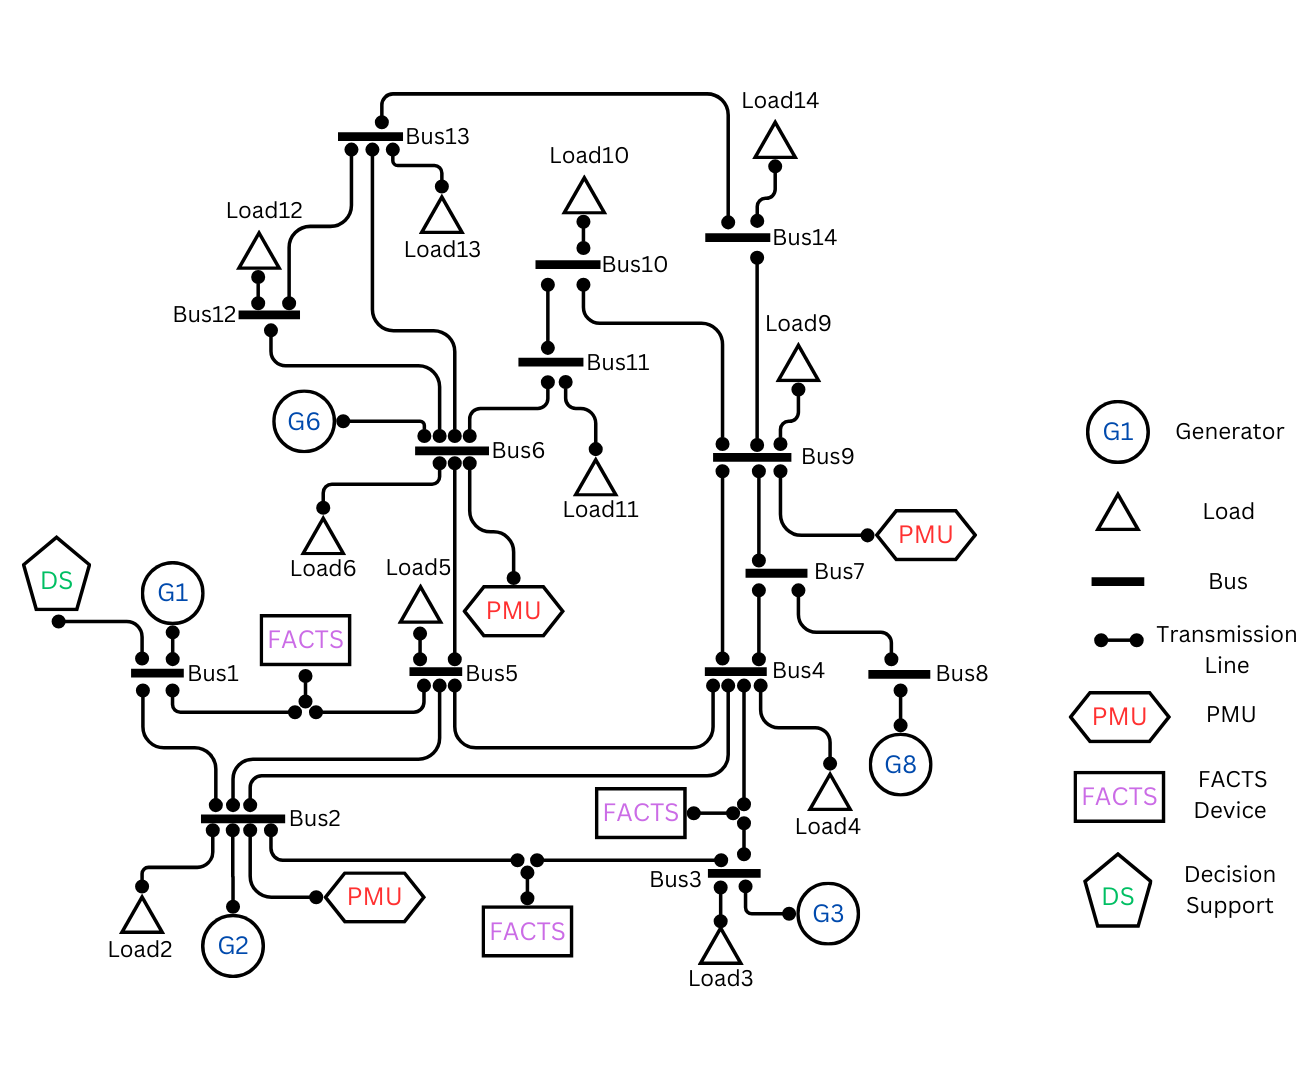
\includegraphics[width=1\linewidth]{images/IEEE-14 smart}
    \caption{IEEE-14 smart grid (adapted from \cite{redacted})}
    \label{fig:IEEE14BUS}
\end{figure}



%replaced (earliest restoration time, number of additional failures, and survivability over the timeline) with rewards. 


\paragraph{Experiment 1: Single-failure}
Among the components in the smart grid, transmission lines, PMUs, FACTS devices, and the decision support system are the ones most likely to fail \cite{song_survey_2013}. Both the 2025 Spain ~\cite{cetinkaya_technical_2025} and 2023 Kenya blackouts \cite{apkenya_aug23, apkenya_dec23, mwangi_kenya_2023} are blackout examples that started with a single-component failure. To replicate the blackout events, we amplified the dependency matrix so that the components are more likely to cause a failure.

For the simulation, we begin with 27 cases to be analyzed for the failure of 27 components, one per case as the initial failure. In each case, we conducted 1,000 Monte Carlo simulation tests and collected the value of the rewards (section \ref{sec:rewards}) over the 27,000 total simulations. For each case, we have also assigned 4 to 2 crews to analyze the impact of available crews on recovery performance. 

\textbf{Table \ref{TB:single}} reports the rewards of each scheme with 2-4 available crews (the best values are marked with \textbf{bold font}).
\begin{table}
\centering
\caption{Experiment 1: single-failure simulation results}
\label{TB:single}
\begin{tabular}{|lrrrr|}
\hline
\rowcolor[HTML]{D9D9D9} 
\multicolumn{1}{|l|}{\cellcolor[HTML]{D9D9D9}Recovery schemes} &
  \multicolumn{1}{l|}{\cellcolor[HTML]{D9D9D9}Rand} &
  \multicolumn{1}{l|}{\cellcolor[HTML]{D9D9D9}Pre-com} &
  \multicolumn{1}{l|}{\cellcolor[HTML]{D9D9D9}Max-cap} &
  \multicolumn{1}{l|}{\cellcolor[HTML]{D9D9D9}Min-cas} \\ \hline
\rowcolor[HTML]{FFFFFF} 
\multicolumn{5}{|c|}{\textbf{2 Crews}} \\ \hline
\multicolumn{1}{|l|}{\cellcolor[HTML]{D9D9D9}Avg. \# of additional failures} &
  \multicolumn{1}{r|}{12} &
  \multicolumn{1}{r|}{\textbf{7}} &
  \multicolumn{1}{r|}{25} &
  10 \\ \hline
\multicolumn{1}{|l|}{\cellcolor[HTML]{D9D9D9}Avg. earliest restoration time} &
  \multicolumn{1}{r|}{18} &
  \multicolumn{1}{r|}{\textbf{13}} &
  \multicolumn{1}{r|}{14} &
  14 \\ \hline
\multicolumn{1}{|l|}{\cellcolor[HTML]{D9D9D9}Recovery Deadline \%} &
  \multicolumn{1}{r|}{\textbf{79.2\%}} &
  \multicolumn{1}{r|}{77.5\%} &
  \multicolumn{1}{r|}{78.4\%} &
  78.1\% \\ \hline
\multicolumn{1}{|l|}{\cellcolor[HTML]{D9D9D9}Coverage} &
  \multicolumn{1}{r|}{86.0\%} &
  \multicolumn{1}{r|}{\textbf{93.8\%}} &
  \multicolumn{1}{r|}{88.3\%} &
  88.6\% \\ \hline
\multicolumn{5}{|c|}{\textbf{3 Crews}} \\ \hline
\multicolumn{1}{|l|}{\cellcolor[HTML]{D9D9D9}Avg. \# of additional failures} &
  \multicolumn{1}{r|}{8} &
  \multicolumn{1}{r|}{6} &
  \multicolumn{1}{r|}{7} &
  7 \\ \hline
\multicolumn{1}{|l|}{\cellcolor[HTML]{D9D9D9}Avg. earliest restoration time} &
  \multicolumn{1}{r|}{11} &
  \multicolumn{1}{r|}{\textbf{10}} &
  \multicolumn{1}{r|}{11} &
  10 \\ \hline
\multicolumn{1}{|l|}{\cellcolor[HTML]{D9D9D9}Recovery Deadline \%} &
  \multicolumn{1}{r|}{\textbf{86.5}\%} &
  \multicolumn{1}{r|}{82.3\%} &
  \multicolumn{1}{r|}{\textbf{86.5}\%} &
  85.8\% \\ \hline
\multicolumn{1}{|l|}{\cellcolor[HTML]{D9D9D9}Coverage} &
  \multicolumn{1}{r|}{96.0\%} &
  \multicolumn{1}{r|}{\textbf{98.8\%}} &
  \multicolumn{1}{r|}{96.7\%} &
  98.3\% \\ \hline
\multicolumn{5}{|c|}{\cellcolor[HTML]{FFFFFF}{\color[HTML]{000000} \textbf{4 Crews}}} \\ \hline
\multicolumn{1}{|l|}{\cellcolor[HTML]{D9D9D9}Avg. \# of additional failures} &
  \multicolumn{1}{r|}{6} &
  \multicolumn{1}{r|}{6} &
  \multicolumn{1}{r|}{6} &
  6 \\ \hline
\multicolumn{1}{|l|}{\cellcolor[HTML]{D9D9D9}Avg. earliest restoration time} &
  \multicolumn{1}{r|}{9} &
  \multicolumn{1}{r|}{9} &
  \multicolumn{1}{r|}{9} &
  9 \\ \hline
\multicolumn{1}{|l|}{\cellcolor[HTML]{D9D9D9}Recovery Deadline} &
  \multicolumn{1}{r|}{90.7\%} &
  \multicolumn{1}{r|}{83.1\%} &
  \multicolumn{1}{r|}{\textbf{91.0\%}} &
  90.4\% \\ \hline
\multicolumn{1}{|l|}{\cellcolor[HTML]{D9D9D9}Coverage} &
  \multicolumn{1}{r|}{99.4\%} &
  \multicolumn{1}{r|}{99.4\%} &
  \multicolumn{1}{r|}{99.5\%} &
  \textbf{99.6\%} \\ \hline
\end{tabular}
\end{table}

\textbf{Figure \ref{fig:singleFail}} reports the recovered system survivability during the simulation process. The axes are adjusted to show the most significant differences between the schemes. 

\begin{figure}
    \centering
    
    \begin{subfigure}[b]{0.4\textwidth}
        \centering
        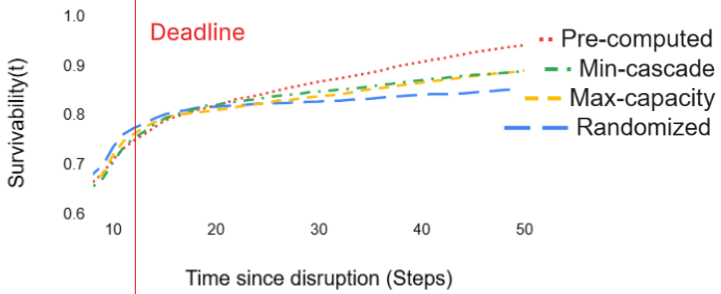
\includegraphics[width=\textwidth]{images/single-2.png}
        \caption{2 repair crews avaliable}
        \label{fig:single-2}
    \end{subfigure}
    \hfill
    \begin{subfigure}[b]{0.4\textwidth}
        \centering
        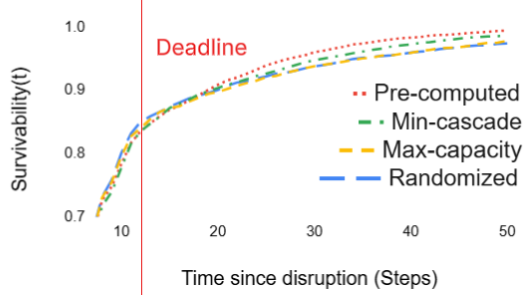
\includegraphics[width=\textwidth]{images/single-3.png}
        \caption{3 repair crews avaliable}
        \label{fig:single-3}
    \end{subfigure}
    \hfill
    \begin{subfigure}[b]{0.4\textwidth}
        \centering
        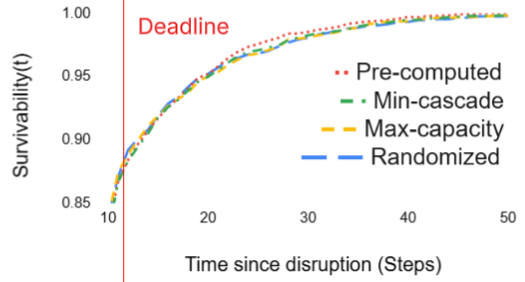
\includegraphics[width=\textwidth]{images/single-4.png}
        \caption{4 repair crews avaliable}
        \label{fig:single-4}
    \end{subfigure}
    
    \caption{Experiment 1: Average survivability over time}
    \label{fig:singleFail}
\end{figure}


As expected, the pre-computed and min-cascade schemes were able to reduce the number of additional failures during the recovery stage. Since we amplified the dependencies, cascading failures are more likely to occur. Especially when there are only a few repair crews available, reducing failures can improve the earliest restoration time, which also shows that the pre-computed scheme is taking the lead after 20 time steps in the system survivability chart (figure \ref{fig:singleFail}. 
Another expectation was that the max-capacity was able to boost the system performance in the early stage, giving the system a slightly higher chance to meet the recovery deadline when there are 3 or 4 crews available. The unexpected thing is that the random scheme provided a greater chance to meet the recovery deadline when there is only 2 crews. As we can see in figure \ref{fig:single-2}, the randomized scheme was dominating the recovered survivability at around 10-20 time steps. The reason is that the max-capacity is going greedy on the survivability and did not focus on mitigating the failures and lost to the random scheme, which is more balanced.

Overall, the simulation of 2-crews was the most intense and showed the highest difference between schemes, as shown in figure \ref{fig:single-2}. However, the 4-crews simulations are mostly the same result because the abundant resource given to repair the system has made the process too short; the cascade will not be likely to occur, and decisions are not significant anymore, as shown in figure \ref{fig:single-4}. \\

\paragraph{Experiment 2: Cyber-attack Scenario}
A cyber-attack can make a power grid blind, confused, or actively dangerous, sometimes all three at once, making them more likely to cause others to fail than normal disruptions. National security relies on electricity, which needs insight from our model for better preparation and protection. The attacker will interrupt the normal operation of the smart devices, causing them to malfunction, and even send malicious commands to manually trigger the imbalance of the power distribution. The 2015 Ukraine blackout~\cite{liang_2015_2017} was one of the recent blackouts caused by cyber-attacks, and the 2025 Spain blackout~\cite{cetinkaya_technical_2025} is under investigation for cyber-attacks. In this experiment, we have also amplified the dependency matrix for that reason.

In our experiment, 3 of the smart devices with the highest probability of failure propagation are assumed to be attacked as the initial failure. They are PMU devices installed on BUS 6 and 9, along with a FACTS device installed on the power line between BUS 1 and 5. 
\textbf{Table \ref{TB:cyber}} reports the rewards of each scheme with 2-4 available crews.

\begin{table}
\centering
\caption{Experiment 2: cyber-attack simulation results}
\label{TB:cyber}
\begin{tabular}{|lrrrr|}
\hline
\rowcolor[HTML]{D9D9D9} 
\multicolumn{1}{|l|}{\cellcolor[HTML]{D9D9D9}Recovery schemes} &
  \multicolumn{1}{l|}{\cellcolor[HTML]{D9D9D9}Rand} &
  \multicolumn{1}{l|}{\cellcolor[HTML]{D9D9D9}Pre-com} &
  \multicolumn{1}{l|}{\cellcolor[HTML]{D9D9D9}Max-cap} &
  \multicolumn{1}{l|}{\cellcolor[HTML]{D9D9D9}Min-cas} \\ \hline
\rowcolor[HTML]{FFFFFF} 
\multicolumn{5}{|c|}{\textbf{2 Crews}} \\ \hline
\multicolumn{1}{|l|}{\cellcolor[HTML]{D9D9D9}Avg. \# of additional failures} &
  \multicolumn{1}{r|}{29} &
  \multicolumn{1}{r|}{\textbf{14}} &
  \multicolumn{1}{r|}{27} &
  21 \\ \hline
\multicolumn{1}{|l|}{\cellcolor[HTML]{D9D9D9}Avg. earliest restoration time} &
  \multicolumn{1}{r|}{36} &
  \multicolumn{1}{r|}{\textbf{23}} &
  \multicolumn{1}{r|}{31} &
  29 \\ \hline
\multicolumn{1}{|l|}{\cellcolor[HTML]{D9D9D9}Recovery Deadline \%} &
  \multicolumn{1}{r|}{\textbf{53.5\%}} &
  \multicolumn{1}{r|}{48.2\%} &
  \multicolumn{1}{r|}{52.6\%} &
  52.8\% \\ \hline
\multicolumn{1}{|l|}{\cellcolor[HTML]{D9D9D9}Coverage} &
  \multicolumn{1}{r|}{59.4\%} &
  \multicolumn{1}{r|}{\textbf{84.9\%}} &
  \multicolumn{1}{r|}{70.70\%} &
  72.8\% \\ \hline
\multicolumn{5}{|c|}{\textbf{3 Crews}} \\ \hline
\multicolumn{1}{|l|}{\cellcolor[HTML]{D9D9D9}Avg.\# of additional failures} &
  \multicolumn{1}{r|}{16} &
  \multicolumn{1}{r|}{\textbf{12}} &
  \multicolumn{1}{r|}{15} &
  15 \\ \hline
\multicolumn{1}{|l|}{\cellcolor[HTML]{D9D9D9}Avg. earliest restoration time} &
  \multicolumn{1}{r|}{17} &
  \multicolumn{1}{r|}{\textbf{14}} &
  \multicolumn{1}{r|}{17} &
  16 \\ \hline
\multicolumn{1}{|l|}{\cellcolor[HTML]{D9D9D9}Recovery Deadline \%} &
  \multicolumn{1}{r|}{\textbf{73.4\%}} &
  \multicolumn{1}{r|}{54.5\%} &
  \multicolumn{1}{r|}{72.7\%} &
  71.1\% \\ \hline
\multicolumn{1}{|l|}{\cellcolor[HTML]{D9D9D9}Coverage} &
  \multicolumn{1}{r|}{91.4\%} &
  \multicolumn{1}{r|}{\textbf{96.8\%}} &
  \multicolumn{1}{r|}{91.9\%} &
  96.5\% \\ \hline
\multicolumn{5}{|c|}{\cellcolor[HTML]{FFFFFF}{\color[HTML]{000000} \textbf{4 Crews}}} \\ \hline
\multicolumn{1}{|l|}{\cellcolor[HTML]{D9D9D9}Avg.\# of additional failures} &
  \multicolumn{1}{r|}{13} &
  \multicolumn{1}{r|}{\textbf{11}} &
  \multicolumn{1}{r|}{13} &
  13 \\ \hline
\multicolumn{1}{|l|}{\cellcolor[HTML]{D9D9D9}Avg. earliest restoration time} &
  \multicolumn{1}{r|}{13} &
  \multicolumn{1}{r|}{\textbf{12}} &
  \multicolumn{1}{r|}{13} &
  13 \\ \hline
\multicolumn{1}{|l|}{\cellcolor[HTML]{D9D9D9}Recovery Deadline} &
  \multicolumn{1}{r|}{\textbf{82.6\%}} &
  \multicolumn{1}{r|}{55.4\%} &
  \multicolumn{1}{r|}{80.5\%} &
  79.8\% \\ \hline
\multicolumn{1}{|l|}{\cellcolor[HTML]{D9D9D9}Coverage} &
  \multicolumn{1}{r|}{\textbf{99.1\%}} &
  \multicolumn{1}{r|}{98.0\%} &
  \multicolumn{1}{r|}{98.9\%} &
  \textbf{99.1\%} \\ \hline
\end{tabular}
\end{table}

\textbf{Figure \ref{fig:CyberAttack}} reports the recovered system survivability during the simulation process.

\begin{figure}[htbp]
    \centering
    
    \begin{subfigure}[b]{0.4\textwidth}
        \centering
        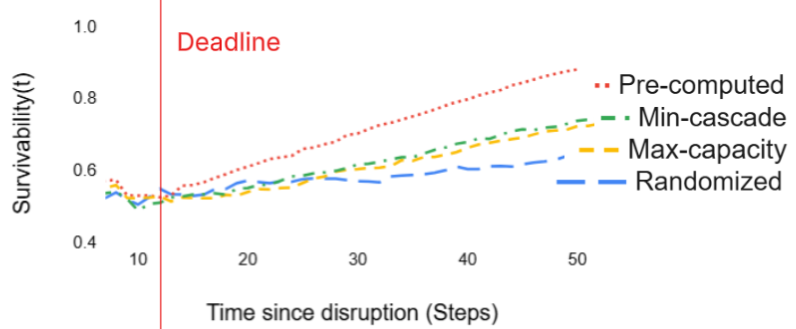
\includegraphics[width=\textwidth]{images/Cyber-2.png}
        \caption{2 repair crews avaliable}
        \label{fig:cyber-2}
    \end{subfigure}
    \hfill
    \begin{subfigure}[b]{0.4\textwidth}
        \centering
        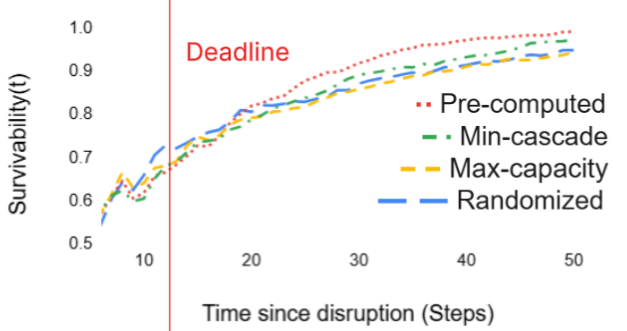
\includegraphics[width=\textwidth]{images/cyber-3.png}
        \caption{3 repair crews avaliable}
        \label{fig:cyber-3}
    \end{subfigure}
    \hfill
    \begin{subfigure}[b]{0.4\textwidth}
        \centering
        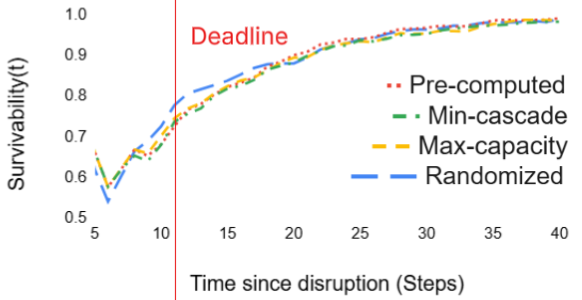
\includegraphics[width=\textwidth]{images/cyber-4.png}
        \caption{4 repair crews avaliable}
        \label{fig:cyber-4}
    \end{subfigure}
    
    \caption{Experiment 2: Average survivability over time}
    \label{fig:CyberAttack}
\end{figure}

Compared to experiment 1, the cyber-attacks have given the system a longer disruption, but they do not impact the system survivability directly. Typically, it takes 5 time steps for the system survivability to go down, whereas the line failure may only take 2 or 3 steps. Because the cyber-attacks will take a few steps for the failure to propagate to the physical layer and actually cause a loss in the service. 
The pre-computed scheme has performed as expected, reducing the additional failures caused by propagation, which shortens the restoration time and increases the survivability recovery rate at the later stage, like after 20 time steps (see figure \ref{fig:CyberAttack}). However, the downside of choosing this scheme is the lowest chance of meeting the recovery deadline in the first 10 time steps. Where the randomized scheme is taking the lead on this merit, but sacrificed the restoration time and experienced many additional failures. Especially in the 2-crew simulation, some trials were unable to be completed within the time horizon (e.g. figure \ref{fig:cyber-2}), leaving the coverage at nearly 60\%. The two dynamic schemes are less extreme in their approach, developing a much more reasonable, tolerable balance between all the rewards, with the max-capacity leaning towards a higher recovery deadline and the min-cascade leaning towards a lower restoration time. \\

\paragraph{Experiment 3: Extreme Weather (Massive Physical Failure)}
On rare occasions, grids could experience massive physical failure due to extreme weather events, such as hurricanes, wildfires, earthquakes, etc. The 2021 North American winter storm~\cite{menati_preliminary_2021} and the 2016 South Australian storm~\cite{jamborsalamati_framework_2018} are significant examples of extreme weather that could cause catastrophic blackouts with cascading failure. Although these events are rare, each time they occur, the system will face a fatal failure with heavy penalties. In situations involving extreme weather or environments, the probability of failure propagation could increase as the components become more vulnerable under such conditions, and the repair time for the components could be longer, as the crews are also working under difficult circumstances. Because failures typically outnumber available crews, dispatch decision schemes become critical.

In our experiment, we construct a storm-passing scenario to evaluate the impact of a extreme weather hazard on the IEEE-14 smart grid (see Fig.~\ref{fig:storm}). 
Since the IEEE-14 test system is a benchmark network defined purely by electrical topology and parameters and does not include real geographic distances or line routing information, the storm trajectory and arrival times are modeled using a synthetic progression rather than physical mileage.
Specifically, the storm is represented as a translating front that sweeps across the network in a fixed direction, and transmission lines are exposed and damaged sequentially according to their relative positions along this path.
The storm advances and affects different regions of the network at discrete time steps. The resulting power line failures occur at different time steps as listed in Table~\ref{TB:storm}, reflecting the progressive impact of the storm as it travels through the system.
\begin{figure}
    \centering
    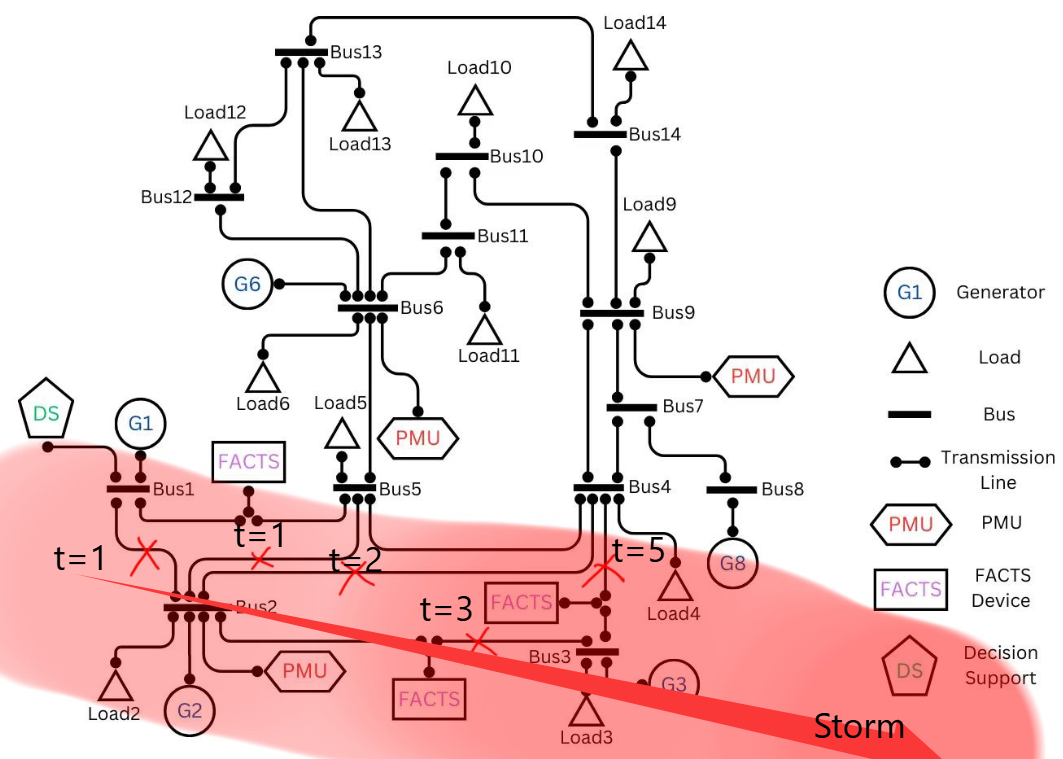
\includegraphics[width=0.7\linewidth]{images/storm_movement.png}
    \caption{Experiment 3: Storm movement map on IEEE-14}
    \label{fig:storm}
\end{figure}
\begin{table}
\centering
\caption{Experiment 3: Power line failure time steps}
\label{TB:storm}
\begin{tabular}{|c|c|}
\hline
Line failed between BUS & At time step (t) \\ \hline
1 \& 2                  & 1                \\ \hline
2 \& 5                  & 1                \\ \hline
2 \& 4                  & 2                \\ \hline
2 \& 3                  & 3                \\ \hline
3 \& 5                  & 5                \\ \hline
\end{tabular}
\end{table}

We have amplified the dependency index to simulate extreme weather conditions in the system. We also increase the average repair time for the components covered in the red area in Figure \ref{fig:storm} by one time step due to the effect of the weather on the crews. We also moved the recovery deadline from the 11th time step to the 15th because the last storm-caused failure occurred at the 5th time step; it would be too cruel to ask the crews to repair the system above 90\% \% of survivability when the repair time for a line could take 3-7 steps. And we also extended the time horizon to 70 time steps, so we can learn more about the recovery process. 

\begin{table}
\centering
\caption{Experiment 3: Extreme weather simulation results}
\label{TB:ExtreW}
\begin{tabular}{|lrrrr|}
\hline
\rowcolor[HTML]{D9D9D9} 
\multicolumn{1}{|l|}{\cellcolor[HTML]{D9D9D9}Recovery schemes} &
  \multicolumn{1}{l|}{\cellcolor[HTML]{D9D9D9}Rand} &
  \multicolumn{1}{l|}{\cellcolor[HTML]{D9D9D9}Pre-com} &
  \multicolumn{1}{l|}{\cellcolor[HTML]{D9D9D9}Max-cap} &
  \multicolumn{1}{l|}{\cellcolor[HTML]{D9D9D9}Min-cas} \\ \hline
\rowcolor[HTML]{FFFFFF} 
\multicolumn{5}{|c|}{\textbf{4 Crews}} \\ \hline
\multicolumn{1}{|l|}{\cellcolor[HTML]{D9D9D9}Avg. \# of additional failures} &
  \multicolumn{1}{r|}{38} &
  \multicolumn{1}{r|}{\textbf{20}} &
  \multicolumn{1}{r|}{28} &
  37 \\ \hline
\multicolumn{1}{|l|}{\cellcolor[HTML]{D9D9D9}Avg. earliest restoration time} &
  \multicolumn{1}{r|}{38} &
  \multicolumn{1}{r|}{\textbf{21}} &
  \multicolumn{1}{r|}{32} &
  34 \\ \hline
\multicolumn{1}{|l|}{\cellcolor[HTML]{D9D9D9}Recovery Deadline \%} &
  \multicolumn{1}{r|}{12.6\%} &
  \multicolumn{1}{r|}{\textbf{19.5\%}} &
  \multicolumn{1}{r|}{15.0\%} &
  2.5\% \\ \hline
\multicolumn{1}{|l|}{\cellcolor[HTML]{D9D9D9}Coverage} &
  \multicolumn{1}{r|}{92.1\%} &
  \multicolumn{1}{r|}{\textbf{98.8\%}} &
  \multicolumn{1}{r|}{97.1\%} &
  94.0\% \\ \hline
\multicolumn{5}{|c|}{\cellcolor[HTML]{FFFFFF}{\color[HTML]{000000} \textbf{5 Crews}}} \\ \hline
\multicolumn{1}{|l|}{\cellcolor[HTML]{D9D9D9}Avg. \# of additional failures} &
  \multicolumn{1}{r|}{31} &
  \multicolumn{1}{r|}{\textbf{21}} &
  \multicolumn{1}{r|}{25} &
  30 \\ \hline
\multicolumn{1}{|l|}{\cellcolor[HTML]{D9D9D9}Avg. earliest restoration time} &
  \multicolumn{1}{r|}{28} &
  \multicolumn{1}{r|}{\textbf{22}} &
  \multicolumn{1}{r|}{25} &
  26 \\ \hline
\multicolumn{1}{|l|}{\cellcolor[HTML]{D9D9D9}Recovery Deadline} &
  \multicolumn{1}{r|}{35.0\%} &
  \multicolumn{1}{r|}{29.8\%} &
  \multicolumn{1}{r|}{\textbf{43.5\%}} &
  21.0\% \\ \hline
\multicolumn{1}{|l|}{\cellcolor[HTML]{D9D9D9}Coverage} &
  \multicolumn{1}{r|}{99.2\%} &
  \multicolumn{1}{r|}{\textbf{99.7\%}} &
  \multicolumn{1}{r|}{99.6\%} &
  99.4\% \\ \hline
\multicolumn{5}{|c|}{\cellcolor[HTML]{FFFFFF}{\color[HTML]{000000} \textbf{6 Crews}}} \\ \hline
\multicolumn{1}{|l|}{\cellcolor[HTML]{D9D9D9}Avg. \# of additional failures} &
  \multicolumn{1}{r|}{26} &
  \multicolumn{1}{r|}{\textbf{21}} &
  \multicolumn{1}{r|}{23} &
  27 \\ \hline
\multicolumn{1}{|l|}{\cellcolor[HTML]{D9D9D9}Avg. earliest restoration time} &
  \multicolumn{1}{r|}{23} &
  \multicolumn{1}{r|}{\textbf{20}} &
  \multicolumn{1}{r|}{22} &
  22 \\ \hline
\multicolumn{1}{|l|}{\cellcolor[HTML]{D9D9D9}Recovery Deadline} &
  \multicolumn{1}{r|}{56.4\%} &
  \multicolumn{1}{r|}{57.5\%} &
  \multicolumn{1}{r|}{\textbf{63.0\%}} &
  50.2\% \\ \hline
\multicolumn{1}{|l|}{\cellcolor[HTML]{D9D9D9}Coverage} &
  \multicolumn{1}{r|}{99.6\%} &
  \multicolumn{1}{r|}{\textbf{99.9\%}} &
  \multicolumn{1}{r|}{99.8\%} &
  99.7\% \\ \hline
\end{tabular}
\end{table}


\textbf{Figure \ref{fig:ExtreWeather}} reports the recovered system survivability during the simulation process.

\begin{figure}[htbp]
    \centering
    
    \begin{subfigure}[b]{0.4\textwidth}
        \centering
        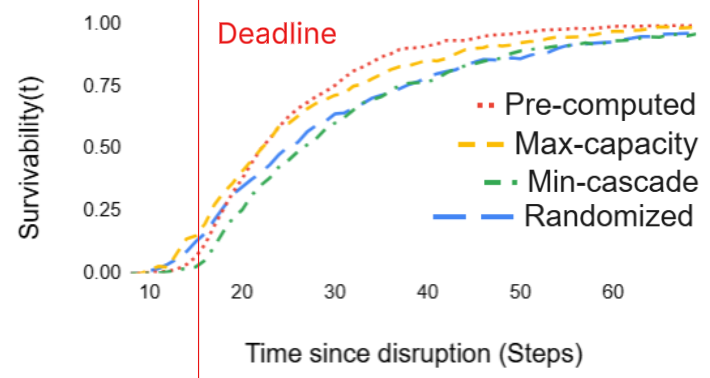
\includegraphics[width=\textwidth]{images/Extre-4.png}
        \caption{4 repair crews avaliable}
        \label{fig:Extre-4}
    \end{subfigure}
    \hfill
    \begin{subfigure}[b]{0.4\textwidth}
        \centering
        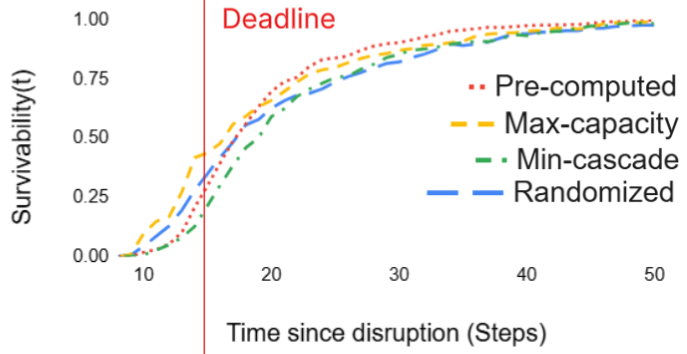
\includegraphics[width=\textwidth]{images/Extre-5.png}
        \caption{5 repair crews avaliable}
        \label{fig:Extre-5}
    \end{subfigure}
    \hfill
    \begin{subfigure}[b]{0.4\textwidth}
        \centering
        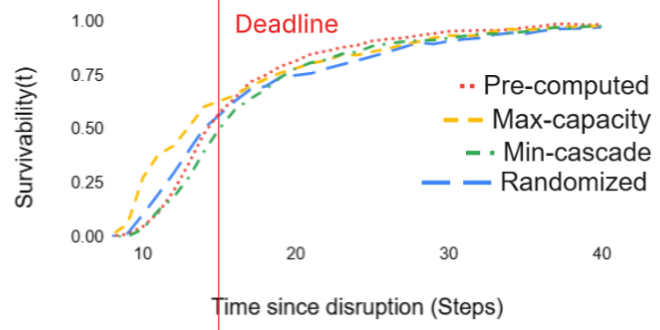
\includegraphics[width=\textwidth]{images/Extre-6.png}
        \caption{6 repair crews avaliable}
        \label{fig:Extre-6}
    \end{subfigure}
    
    \caption{Experiment 3: Average survivability over time}
    \label{fig:ExtreWeather}
\end{figure}


Compared to other experiments, this one has a higher loss of survivability in the early stage (usually takes 10 time steps to start recovering from 3+ line failures), and it takes more crews to win the race against cascading failure, so we assign more available crew than the previous experiment. In reality, the electric company may request help from neighboring states to assist them with extra crews during an event like this. 

As expected, the pre-computed scheme was able to minimize the additional failure, which leads to the shortest time to restoration and effective bounce back after 20 time steps as before (see figure \ref{fig:ExtreWeather}). The max-capacity was able to take the lead this time on recovering the system survivability before the deadline, and we could see the significant gap between max-capacity and every other scheme in the early 10-20 time steps in figure \ref{fig:Extre-5} and \ref{fig:Extre-6}.


\paragraph{Experiment 4: IEEE-30 double-failure}
The IEEE-30 system is used for demonstrating the scalability of the proposed model. The original IEEE-30 has 41 lines, 30 BUS, and 24 loads.
%We have created IEEE-30 smart from the original system by adding 6 PMUs on BUS 1,5,10,12,15,27; and 5 FACTS on lines between BUS 6 \& 8, 8 \& 28, 22 \& 28, 27 \& 28, 27 \& 30; for the best observability and configurability. 
\textbf{Figure \ref{fig:IEEE30}} described the IEEE-30 smart grid system used for our case study. We are using the same method to calculate the dependency for IEEE-30 and the same repair time for each component based on their type. The only difference is the system survivability calculation. MATLAB with the PSAT toolbox was embedded into Google Colab to solve the system survivability for when the system has $\leq 3$ failed lines; otherwise, the survivability will be 0 (same as IEEE-14). Using the PSAT toolbox is a compromise to the size of IEEE-30. Since there are 41 lines, 5 FACTS devices, and a decision support, there could be a $2^{46} \approx 10^{13}$ unique state, which is impossible to make and store a search table in our machine. The only downside of using embedded PSAT is the long execution time (typically 10 seconds per check), much longer than using a search table ($< 1$ second). %Perhaps artificial intelligence techniques could be used to speed up the power flow calculation in our future work. 
For that reason, we decided to put together one simulation with 100 trials, with a time horizon at 50 time steps.

To systematically capture the race between failure propagation and recovery efforts, we design a double-failure scenario on the IEEE-30 test system. Because the IEEE-30 smart grid is larger and structurally more redundant than IEEE-14, its inter-component dependencies are comparatively weaker; as a result, the failure of a single component is more readily absorbed by the network. Consequently, we select a two-component initial failure for our experimental setup. From the 53 candidate components in the system, we designate transmission lines 23 and 6 (see Figure \ref{fig:IEEE30}) as the initial failure. This choice is informed by an importance analysis performed on all IEEE-30 components using the \emph{critical} method introduced in \cite{redacted5}. That analysis identified these two lines as among the most likely to induce extensive fault propagation and to exert the largest adverse effect on system survivability within the average recovery horizon of five time steps. And we have also amplified the dependency matrix between the components during simulation so the cascading failures are more likely to happen. 

\begin{figure}
    \centering
    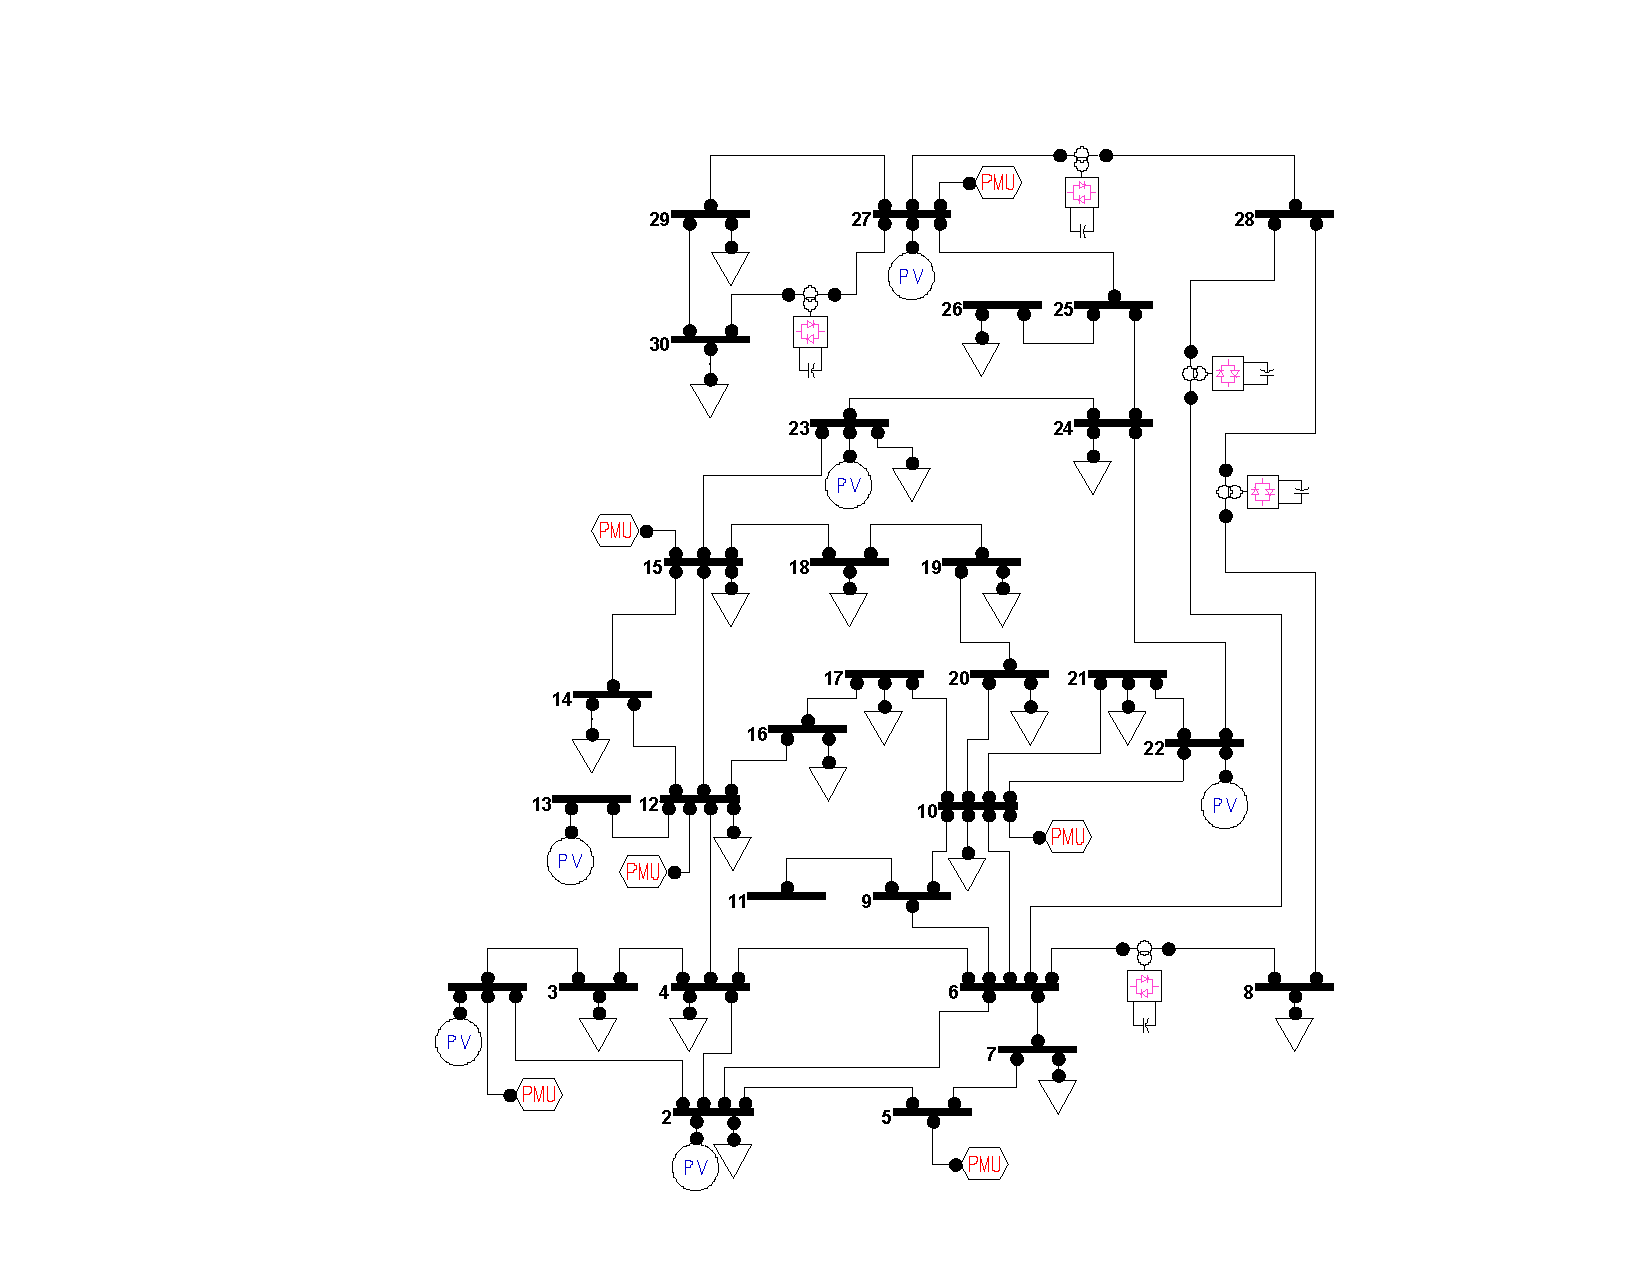
\includegraphics[width=0.6\linewidth]{images/ieee30.pdf}
    \caption{IEEE-30 smart grid adopted from \cite{redacted5}}
    \label{fig:IEEE30}
\end{figure}

\begin{table}
\centering
\caption{Experiment 4: IEEE-30 double-failure simulation results}
\label{TB:30results}
\begin{tabular}{|lrrrr|}
\hline
\rowcolor[HTML]{D9D9D9} 
\multicolumn{1}{|l|}{\cellcolor[HTML]{D9D9D9}Recovery schemes} &
  \multicolumn{1}{l|}{\cellcolor[HTML]{D9D9D9}Rand} &
  \multicolumn{1}{l|}{\cellcolor[HTML]{D9D9D9}Pre-com} &
  \multicolumn{1}{l|}{\cellcolor[HTML]{D9D9D9}Max-cap} &
  \multicolumn{1}{l|}{\cellcolor[HTML]{D9D9D9}Min-cas} \\ \hline
\rowcolor[HTML]{FFFFFF} 
\multicolumn{5}{|c|}{\textbf{2 Crews}} \\ \hline
\multicolumn{1}{|l|}{\cellcolor[HTML]{D9D9D9}Avg. \# of additional failures} &
  \multicolumn{1}{r|}{12} &
  \multicolumn{1}{r|}{14} &
  \multicolumn{1}{r|}{\textbf{8}} &
  \textbf{8} \\ \hline
\multicolumn{1}{|l|}{\cellcolor[HTML]{D9D9D9}Avg. earliest restoration time} &
  \multicolumn{1}{r|}{14} &
  \multicolumn{1}{r|}{14} &
  \multicolumn{1}{r|}{\textbf{12}} &
  \textbf{12} \\ \hline
\multicolumn{1}{|l|}{\cellcolor[HTML]{D9D9D9}Recovery Deadline \%} &
  \multicolumn{1}{r|}{72\%} &
  \multicolumn{1}{r|}{72\%} &
  \multicolumn{1}{r|}{72\%} &
  72\% \\ \hline
\multicolumn{1}{|l|}{\cellcolor[HTML]{D9D9D9}Coverage} &
  \multicolumn{1}{r|}{90\%} &
  \multicolumn{1}{r|}{90\%} &
  \multicolumn{1}{r|}{\textbf{100\%}} &
  \textbf{100\%} \\ \hline
\multicolumn{5}{|c|}{\cellcolor[HTML]{FFFFFF}{\color[HTML]{000000} \textbf{3 Crews}}} \\ \hline
\multicolumn{1}{|l|}{\cellcolor[HTML]{D9D9D9}Avg. \# of additional failures} &
  \multicolumn{1}{r|}{19} &
  \multicolumn{1}{r|}{23} &
  \multicolumn{1}{r|}{\textbf{9}} &
  \textbf{9} \\ \hline
\multicolumn{1}{|l|}{\cellcolor[HTML]{D9D9D9}Avg. earliest restoration time} &
  \multicolumn{1}{r|}{13} &
  \multicolumn{1}{r|}{15} &
  \multicolumn{1}{r|}{\textbf{10}} &
  \textbf{10} \\ \hline
\multicolumn{1}{|l|}{\cellcolor[HTML]{D9D9D9}Recovery Deadline} &
  \multicolumn{1}{r|}{\textbf{76\%}} &
  \multicolumn{1}{r|}{72\%} &
  \multicolumn{1}{r|}{72\%} &
  72\% \\ \hline
\multicolumn{1}{|l|}{\cellcolor[HTML]{D9D9D9}Coverage} &
  \multicolumn{1}{r|}{87\%} &
  \multicolumn{1}{r|}{86\%} &
  \multicolumn{1}{r|}{\textbf{100\%}} &
  \textbf{100\%} \\ \hline
\multicolumn{5}{|c|}{\cellcolor[HTML]{FFFFFF}{\color[HTML]{000000} \textbf{4 Crews}}} \\ \hline
\multicolumn{1}{|l|}{\cellcolor[HTML]{D9D9D9}Avg. \# of additional failures} &
  \multicolumn{1}{r|}{27} &
  \multicolumn{1}{r|}{33} &
  \multicolumn{1}{r|}{13} &
  \textbf{11} \\ \hline
\multicolumn{1}{|l|}{\cellcolor[HTML]{D9D9D9}Avg. earliest restoration time} &
  \multicolumn{1}{r|}{14} &
  \multicolumn{1}{r|}{16} &
  \multicolumn{1}{r|}{11} &
  \textbf{10} \\ \hline
\multicolumn{1}{|l|}{\cellcolor[HTML]{D9D9D9}Recovery Deadline} &
  \multicolumn{1}{r|}{\textbf{76\%}} &
  \multicolumn{1}{r|}{72\%} &
  \multicolumn{1}{r|}{72\%} &
  72\% \\ \hline
\multicolumn{1}{|l|}{\cellcolor[HTML]{D9D9D9}Coverage} &
  \multicolumn{1}{r|}{84\%} &
  \multicolumn{1}{r|}{79\%} &
  \multicolumn{1}{r|}{97\%} &
  \textbf{99\%} \\ \hline
\end{tabular}
\end{table}

\begin{figure}[htbp]
    \centering
    
    \begin{subfigure}[b]{0.4\textwidth}
        \centering
        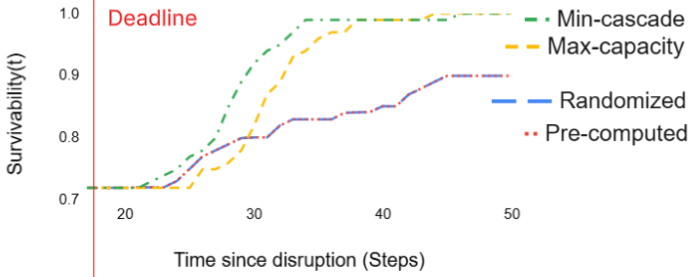
\includegraphics[width=\textwidth]{images/IEEE30-2.png}
        \caption{2 repair crews avaliable}
        \label{fig:30-2}
    \end{subfigure}
    \hfill
    \begin{subfigure}[b]{0.4\textwidth}
        \centering
        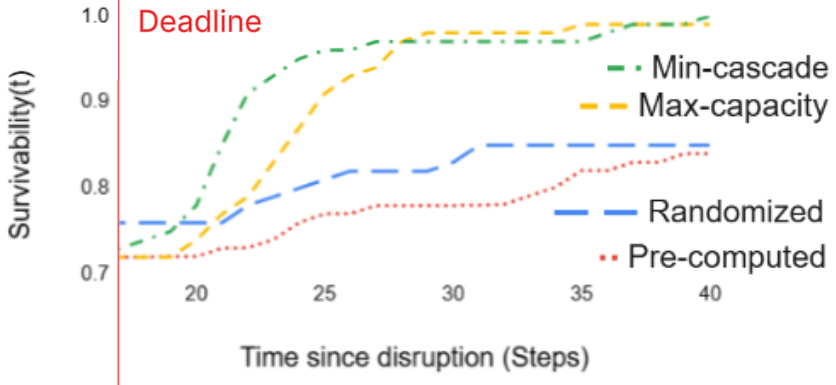
\includegraphics[width=\textwidth]{images/IEEE30-3.png}
        \caption{3 repair crews avaliable}
        \label{fig:30-3}
    \end{subfigure}
    \hfill
    \begin{subfigure}[b]{0.4\textwidth}
        \centering
        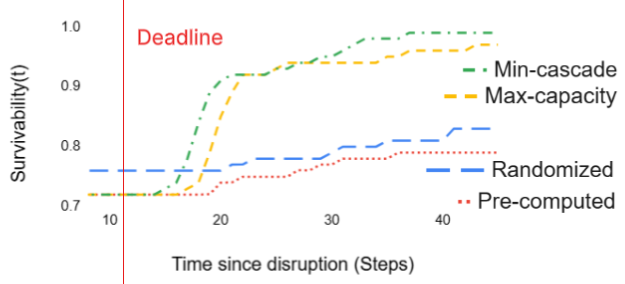
\includegraphics[width=\textwidth]{images/IEEE30-4.png}
        \caption{4 repair crews avaliable}
        \label{fig:30-4}
    \end{subfigure}
    
    \caption{Experiment 4: Average survivability over time}
    \label{fig:30-result}
\end{figure}

The result of this experiment is unexpectedly different from any IEEE-14 result. Since IEEE-30 is much larger and structurally more complex than IEEE-14, we have examined the state transitions within the simulation and discovered an interesting phenomenon. As we increase the number of repair crews, the additional failures and earliest restoration time increase in some cases,  especially in pre-computed schemes. The reason for causing this phenomenon is behind the failure propagation. Some components have much stronger dependencies (higher likelihood to fail or cause failure); strong dependencies would take longer for the system to adapt and absorb, and the weak dependencies could be much easier to deal with (as shown in equation \ref{eq:pij}, the dependencies are decreasing exponentially). However, if a low-dependency component is constantly getting repaired and fails again, the system will have to absorb the dynamics once more, which is more likely to cause failure than leaving the component failed. Similar to things that happened in the 2023 Kenya blackout, the repairs didn't help with the power shortage but expanded the outage to more areas. 
The pre-computed scheme somehow made decisions that aggravated this phenomenon and generated a worse result when more crews were available. So the additional failures increase as shown in table \ref{TB:30results}, and it could delay the restoration time and even lower the coverage of the simulation. On the chart (figure. \ref{fig:30-result}), we can see the recovery rate of the pre-computed scheme is getting worse and worse as well. While the Min-cas was focusing on the smart devices before the lines, so the smart layer got restored first, so it can help reconfigure the power flow to a stable state. And the max capacity focused on the physical layer by restoring the lines first, which gave the systems more connection, thus reducing the additional failures. The randomized is similar to the pre-computed scheme that didn't focus on one layer of the system; just randomly doing fixes will still bring the system many additional failures. However, the random scheme was able to restore the most performance before the deadline, and we can also see that it has a higher average survivability before the 20th time step (shown in figure \ref{fig:30-result}) and the min-cascade is dominating the rest of the timeline, which is similar to the pre-computed scheme in IEEE-14 experiments. 

The main purpose of this experiment is to show the scalability of the model, that it can apply to larger network systems. One way to show that is by comparing the simulation time; the IEE-30 takes much longer than the IEEE-14 due to the survivability check with PSAT. The IEEE-14 takes about 0.5-1 hrs to finish simulation with Google Colab with runtime type set to CPU, using 1-2 GB of RAM and 20-25 GB of disk.
The IEEE-30 takes about 2-4 hrs to finish simulation under the same environment (with 4 hrs being with using the max-capacity method, as it requires a survivability check as well) and about the same space. If the survivability check was disabled for IEEE-30, it only takes about 0.2 hrs to complete the simulation. Although it is only doing 100 simulations, whereas IEEE-14 is doing 1,000 simulations, the result is showing the scalability of the model and capability for larger systems if a fast survivability check is available.  

\section{Conclusions and Future Work}

This paper proposes a mathematical model to analyze the race between cascading failure and recovery efforts in a complex networked system. Our model predicts failure propagation with consideration of the effect of recovery actions and facilitates evaluation of system survivability after each action, all of which are crucial to decision support during recovery.

To illustrate the utility of our model, we carried out case studies on respective simulated smart grids based on the IEEE-14 and IEEE-30 test systems. Given a number of recovery schemes that differ in objective, for example maintaining service capacity vs. limiting failure propagation vs. achieving the fastest recovery, the experiments collectively demonstrated that our model can provide decision support during recovery by elucidating differences between their outcomes.

Our model is not limited to power grids. Given the topology and component-level information, our model can be used to analyze recovery schemes for other networked systems. Examples include water distribution networks and transportation systems. Other directions for extending the model to include consideration of partially observable component states, and concurrent component failures that are independent of an ongoing cascade. More refined repair time distributions that incorporate logistics-based time estimation, as well as allowing for partially or completely unsuccessful recovery actions, are among potential enhancements to the model.

%\section{Acknowledgment}
%\thanks{Funding from NSF DUE-1742523 and DUE-2221559 and Department of Education awards P200A180095 and P200A210121 is gratefully acknowledged.}

\bibliographystyle{IEEEtran}
\bibliography{export-data.bib}
%SSS - export-date is still blank

\end{document}
